% -*- mode: latex; tab-width: 4; indent-tabs-mode: nil -*-
%
% Copyright (C) 2012-2015 Marco Craveiro <marco.craveiro@gmail.com>
%
% This program is free software; you can redistribute it and/or modify
% it under the terms of the GNU General Public License as published by
% the Free Software Foundation; either version 3 of the License, or
% (at your option) any later version.
%
% This program is distributed in the hope that it will be useful,
% but WITHOUT ANY WARRANTY; without even the implied warranty of
% MERCHANTABILITY or FITNESS FOR A PARTICULAR PURPOSE. See the
% GNU General Public License for more details.
%
% You should have received a copy of the GNU General Public License
% along with this program; if not, write to the Free Software
% Foundation, Inc., 51 Franklin Street, Fifth Floor, Boston,
% MA 02110-1301, USA.
%
\documentclass{book}
\usepackage{qlbook}

%
% packages
%
\usepackage{lettrine}
\usepackage{graphicx}
\usepackage{hyperref}
\usepackage{listings}

% Title setup.
\tolerance=1000
\date{\today}
\author{Marco Craveiro}
\title{Dogen: The Domain Generator}

\hypersetup{
  pdfkeywords={},
  pdfsubject={},
  pdfcreator={Emacs 24.5.1 (Org mode 8.2.10)}}

\begin{document}

\maketitle

%
% Colophon
%
\newpage
\pdfbookmark[0]{Colophon}{Colophon}
\section*{}
\pagestyle{empty}
%\chapter*{}
\vfill
\begingroup
\footnotesize
\parindent 0pt
\parskip \baselineskip

\textcopyright{} 2012-2015 Marco Craveiro \\
All rights reserved.

Revision \textbf{DRAFT}. Generated for Dogen v${DOGEN_VERSION}, git
commit ${CURRENT_GIT_COMMIT}.

This book was typeset with \LaTeXe. It uses a slightly modified
version of the \textit{QL Book} style developed by Luigi Ballabio.
Download the \textit{QL Book} style at
\url{http://www.implementingquantlib.com/p/the-book.html}.

\par Permission is granted to copy, distribute and/or modify this
document under the terms of the GNU Free Documentation License,
Version 1.2 or any later version published by the Free Software
Foundation; with no Invariant Sections, no Front-Cover Texts, and no
Back-Cover Texts. A copy of the license is included in the appendix
entitled ``GNU Free Documentation License.''

\endgroup
\clearpage

\newpage

\setcounter{tocdepth}{2}
\tableofcontents
\listoffigures
\listoftables

\chapter*{Preface}

\epigraph{Le mieux est l'ennemi du bien.}{Voltaire}

\epigraph{First write the code generator; don't worry about the code,
  it will write itself.}{\emph{author}}

\epigraph{Malembe, Malembe.}{Angola proverb}

\section*{About This Document}

This document is the official manual for Dogen. Dogen~--- the domain
generator~--- is a suite of code generation tools designed
specifically to target domain models. Dogen was created to make the
modeling process simpler: the user creates a domain model using a UML
tool and the tools provided by Dogen use it to generate its source
code representation. The generated code contains most of the services
required from a typical C++ domain object such as serialisation,
hashing, io (streaming) and so on.

If you are reading a printed copy of this manual, you can always
access the latest version online:

\begin{itemize}
\item \url{https://github.com/kitanda/dogen/blob/master/doc/manual/manual.org}
\end{itemize}

\section*{More Information}

You can find the latest source code for Dogen at the official
repository in GitHub:

\begin{itemize}
\item \url{https://github.com/kitanda/dogen}
\end{itemize}

There is also a mirror in BitBucket:

\begin{itemize}
\item \url{https://bitbucket.org/marco_craveiro/dogen/overview}
\end{itemize}

Continuous builds are available via CDash:

\begin{itemize}
\item \url{http://my.cdash.org/index.php?project=Dogen}
\end{itemize}

You can find details on the ongoing work in the Agile folder (look for
the latest sprint):

\begin{itemize}
\item \url{https://github.com/kitanda/dogen/tree/master/doc/agile}
\end{itemize}

\part{Theory}

In this part we describe the philosophical underpinnings behind Dogen,
its internal architecture and assorted aspects around its development.

\chapter{Fundamental Building Blocks}

\lettrine{T}{his} section focuses on the more abstract aspects of
Dogen.

\section{The Question}

Dogen is largely the result of exploring a simple question: what
portion of the objects required to model a problem domain is
generatable by a program, such that the generated code is as good as,
or better than, code crafted by humans? This question stems from many
years of looking at object models and their limitations, in various
incarnations.

One of the main problems one often finds in production code is a lack
of a large number of simple but very useful ``facilities'', which all
objects on all domain models should have. For instance, a simple way
of dumping current state to a stream, in a format that can be
understood by external tools. Developers tend to add facilities like
these on a haphazard sort of manner, because it is laborious and not
particularly exciting functionality to work on. By the time the domain
model has matured, it is often too late to find time for it.

A further observation is that a large part of the objects required to
model a problem domain have fairly straightforward behaviour; in many
cases they are but glorified structs with a few trivial abilities
bolted on, such as serialisation and hashing. A lot of programmer time
is taken on generating getters, setters, serialisation code and so
on. It is easy to get sloppy with this kind of code because its so
repetitive.

Trying to answer this question led us along a road less travelled by
regular developers: the world of \emph{meta}.

\section{On Models and Modeling}

Before we go too much further, it is important to clarify what is
meant by a model. After all, programming is the art of refining
abstractions. It is the programmer's job to create a set of constructs
that represent concepts found in the problem domain; and to get those
concepts to cooperate successfully in producing work that is defined
as useful by something or someone~--- that is, to solve a
\emph{problem} in the problem domain. Together, this collection of
concepts \emph{models} the problem domain because it is a
representation of a subset of the problem domain inside of the
computer. One may even further qualify it as a ``special'' kind of
model~--- a \emph{domain model}. \emph{Domain modeling} is then the
activity of identifying a set of \emph{domain types} that describe the
domain in question via their properties, relationships and behaviours.

Whilst all of this may seem pretty obvious, it is a terrain rife for
misconceptions. First, in a strict sense, all models are ``domain
models'' because they exist as a model of a domain somewhere. However,
in practice, one tends to make an important distinction between the
domain we're interested in at a given point in time, and all other
``helper models'' that are there to just give us a hand. It is in this
context that we say that ``domain models'' are ``special''. Second, it
is important to notice that \emph{the} domain model is a conceptual
entity. It manifests itself in a myriad of representations~--- UML
diagrams, source code, database schemas and so on~--- but none of
these representations \emph{is} the domain model. For instance, if you
were to ``write down the domain model'' (via specifications or
otherwise), you would do nothing but create yet another such
representation, this time expressed in the medium of natural
language. The logical consequence is twofold: there is no such thing
as a ``complete'' representation of the domain model~--- it is only
``complete'' insofar as the purposes for which it has been created are
satisfied; and any representation is highly sensitive to the
properties of the medium it is expressed in.

To ram the point home: there is no such thing as the \emph{better} or
\emph{best} representation of a domain model; it only makes sense to
make comparative statements of this kind when there is an objective
task against which two or more representations can be evaluated. Any
non-trivial software system requires several representations, each
specialising on a particular area, and transformations between
representations are required.

We should now be able to drop the ``domain'' prefix and refer to just
``models'' or ``modeling'' and presume that all of the above is implied.

You may think that we're sliding down the conceptual slippery-slope
for no good reason. As we shall see, these fundamental ideas are
important in shaping how you use Dogen. For now you can start to think
of it as the tooling infrastructure that tries to automate as much as
possible the transformation of one representation of a model into
another.

\section{On Code Generation and Meta-Models}

Dogen didn't come to exist in a vacuum, but rather on a continuum, and
the continuum had it's genesis very early on. In fact, the concept of
programs that generate programs is probably as old as computer science
itself: it certainly was a common feature in the days of machine code
and assembler code programming. These ideas were incorporated in early
languages such as LISP, where there was a blurring of the lines
between hand crafted source code and machine generated source
code. Sadly, these progressive thoughts faded into the background as
the C family of languages took front stage.

It's not as if code generation disappeared~--- it just went into
hiding. In fact, today there are many widely used tools in the Open
Source ecosystem that generate code:

\begin{itemize}
\item \href{https://developers.google.com/protocol-buffers/}{Google Protocol Buffers}
\item \href{http://www.codesynthesis.com/products/odb/}{ODB}: C++ Object-Relational Mapping (ORM)
\item \href{http://www.codesynthesis.com/products/xsde/}{eXSD}: XSD/e: XML for Light-Weight C++ Applications
\item \href{http://msdn.microsoft.com/en-us/library/windows/desktop/aa367300(v\%3Dvs.85).aspx}{MIDL}: COM IDL compiler
\item and many more.
\end{itemize}

Each of these tools are designed to do a specific task and to do it
well, hiding as much as possible of the code generation details from
the end user. We call these \emph{special purpose} code generators~---
although, as we shall see, in a sense all code generators are special
purpose. The code generated by these tools contains both the data
structures they require as well as hard-coded behaviour associated
with them: how to read and write them from raw storage (in the case of
Protocol Buffers), how to read and write them from the database (ODB),
and so on. One is not expected to tamper with the generated code.

All code generators have an internal set of data structures that
represent the entities to generate~--- explicitly or implicitly. These
data structures are known as the \emph{meta-model}. Meta-models are a
class of domain models that focus on describing domain models
themselves. They allow code to introspect and to think about code; to
reflect. In this form, code generation is simply the transformation of
a model, described in one such representation (the meta-model) into
another representation (the source code), following the rules laid out
by the grammar of a programming language. The richer the meta-model,
the more expressive the generated code can be~--- and vice-versa. It
is in this sense that certain classes of code generators are called
special purpose, because they have meta-models that are very focused,
designed only for the task at hand. Don't think of this as a
disadvantage though: there is a price to pay in complexity for every
ounce of flexibility, so its best to have simple code that does one
thing and does it well.

Nevertheless, meta-models can be useful in a more general form when
designing software applications: they can allow one to reason about
the structure of the code. One of the most common meta-models in
existence is
\href{http://en.wikipedia.org/wiki/Unified_Modeling_Language}{UML}. UML
is used widely in the industry and there are many tools that can be
used to generate source code from UML diagrams. It is simultaneously
ubiquitous~--- it is available everywhere~--- and complete~--- that
is, as a meta-model, it defines a extensive list of concepts for
pretty much any aspect of programming. Thus it is common for tools to
take a UML representation and use it to generate source code; as
examples of Open Source tools that can generate source code from a UML
diagram see:

\begin{itemize}
\item \href{http://dia2code.sourceforge.net/}{dia2code}
\item \href{http://umbrello.kde.org/}{Umbrello} (see \href{http://docs.kde.org/development/en/kdesdk/umbrello/code-import-generation.html}{this} for code generation)
\end{itemize}

In a sense one, one may think of these tools as \emph{general purpose}
code generators because they output code that is not tied up to any
specific purpose, other than to model the problem domain. Unlike the
special purpose tools, the generated code is very much skeleton code,
code that adds little in terms of behaviour. This is all as it should
be: the more specific your intent is, the more the code generator can
do for you and, conversely, the less specific your intent is, the less
helpful the code generator can be.

The astute reader would have already devised a simple solution to the
behaviour conundrum: nothing stops us from modeling the signatures of
methods in the meta-model~--- after all UML provides us with all the
required machinery~--- and then hand-craft an implementation for these
methods. Indeed there are code generators which permit such workflows;
they are known as \emph{merging code generators}. The merging aspect
comes from the fact that the code generator must be able to
distinguish between the hand-crafted code and the machine generated
code in order to handle meta-model updates.

So these are three key themes for Dogen: special purpose code
generation, general purpose code generation and merging code
generation. But before we can proceed, we need to add one more actor
to the scene.

\section{On Domain Driven Design}

One of the main problems facing software engineers working on large
systems is the need to clearly separate business rules from
scaffolding code. In many ways, this need originates from the long
forgotten days when the word \emph{Application} was coined: the use of
computer science \emph{applied} to a specific problem to provide an
automated solution to the set of people with the problem~--- the
\emph{users}. During the process of development, users will provide
all sorts of insights into what it is they want solved, and these are
ultimately captured in code (see
\href{http://www.developerdotstar.com/mag/articles/PDF/DevDotStar_Reeves_CodeAsDesign.pdf}{Jack
  Reeves' essays} on this topic). Code will also be made up of reading
and writing records to a database, socket communication, reading and
writing to file and so on; the challenge then is to avoid obscuring
the former while dealing with the latter.

Many people have thought deeply about this dichotomy. Arguably, the
most significant advance was made by Eric Evans with his seminal book
\href{http://www.amazon.co.uk/Domain-driven-Design-Tackling-Complexity-Software/dp/0321125215}{Domain-Driven
  Design}: Tackling Complexity in the Heart of
Software\cite{evans2004domain}. Domain Driven Design (DDD) is a
software engineering methodology that places great emphasis on
understanding the problem domain and, coupled with Agile, it provides
a great platform for iterative improvements both to the understanding
and to its expression in code. DDD focuses on defining a clear and
concise domain model~--- a set of classes and relationships that model
the insights provided by the users and domain experts in general. It
also explains the difference between the conceptual domain model and
myriad of representations: UML diagrams, specification documents, oral
conversations and, most importantly, source code.

\section{Adding It All Together}

The key idea behind Dogen is that all of the aspects we described up
til now are deeply interrelated. That is to say that we store deep
knowledge about the domain in meta-models, which tend to be
represented graphically~--- say in UML class diagrams; and we do so
because these representations provide a quick and yet expressive way
to communicate domain knowledge. But those very same documents are~---
or can be made~--- sufficiently complete to be used as a basis for the
code generation of skeleton code by some general purpose code
generation tool. Furthermore, there are a large number of facilities
that are required of most domain models, and these can be thought of
as special purpose extensions to such a general purpose tool; and,
finally, that which cannot be code generated can be manually added and
merged in. And thus all the strands are weaved into a single tool.

Lets return to the ``facilities'' required by all domain models. What
do we mean exactly? Well, ODB and the like already hinted at some of
the things one may wish to do with C++ objects~--- persist them in a
database~--- but there are other even more fundamental requirements:

\begin{itemize}
\item the ability to support getters and setters, hashing,
  comparisons, assignment, move construction and many other
  fundamental behaviours;
\item the ability to dump the current state of the object to a C++
  stream in a format that is parsable by external tools (like say
  JSON);
\item the ability to generate
  \href{http://stackoverflow.com/questions/5140475/how-to-write-native-c-debugger-visualizers-in-gdb-totalview-for-complicated-t}{debugger
    visualisers};
\item the ability to serialise and deserialise objects using a
  multitude of technologies such as
  \href{http://download.oracle.com/otn_hosted_doc/coherence/353CPP/index.html}{POF},
  \href{http://www.boost.org/doc/libs/1_55_0/libs/serialization/doc/index.html}{Boost
    Serialisation}, \href{https://github.com/hjiang/jsonxx}{JSON},
  \href{http://libxmlplusplus.sourceforge.net/}{XML} and many others;
\item the ability to generate objects populated with random data for
  testing;
\item \ldots{}
\end{itemize}

And on and on. Other languages would have a similar list~--- if
perhaps not so extensive, as the use of reflection already allows them
to satisfy some of these use cases generically, at the cost of
performance. The more we looked, the more boilerplate code we
found~--- code that could easily be generated for the vast majority of
the cases. There are, of course, quite a few corner cases which are
just too hard to automate, but they can easily be manually coded.

The picture that emerges from this
\href{http://en.wikipedia.org/wiki/Thought_experiment}{gedankenexperiment}
is some kind of ``cyborg'' coding. A type of programming where any and
all aspects that can be reduced to a set of rules~--- applicable to
instances of the meta-model~--- are implemented as extensions of the
code generator; and this process of extension continues over time, as
the meta-model becomes more and more expressive.

Dogen is an attempt to create such a tool. As we are C++ developers we
started off by trying to implement the vision as a C++ tool; but the
notions are general enough that they would apply to any programming
language.

\chapter{The Architecture}

\lettrine{D}{ogen} is made up of a large number of domain
models. These fall into two broad categories: \emph{test models} and
\emph{main models}. Test models are models we created specifically to
test some aspect of code generation~--- such as say inheritance~---
and whose code is not used by the main binary. The main models are
what really makes up the application.

Lets look at each of these in more detail.

\section{Main Models}

Dogen is made up of a number of main models, hooked together in
different ways. But before we look into the main models, we need to
understand the users of these models: the suite of tools.

\subsection{Dogen as a suite of tools}

Dogen is really just a suite of different tools that are related to
code generation. Since we could not think of natural names to use,
sewing was used as a theme. The naming scheme uses a couple of simple
conventions:

\begin{itemize}
\item top-level libraries that implement a tool use the infinitive
  form of the verb (minus the ``to'', where applicable).
\item where applicable, we may have an executable binary that wraps
  the top-level library. In this case, we use the noun closest to the
  verb~--- even if in some cases we have to ``nounify'' the verb.
\end{itemize}

At present, the following tools exist or have been planned:

\begin{center}
\begin{tabular}{llll}
Tool Name & Top-level library & Status & Description\\
\hline
knitter & knit & started & Code-generation of models.\\
stitcher & stitch & started & Basic text-templating support (similar to T4).\\
darner & darn & vision & Generates JSON from Dia diagrams\\
 & needle & vision & Library with supporting code, used by generated models.\\
patch & patcher & vision & Updates a dia Diagram given a C++ code base.\\
 & quilt & vision & Native domain model representation\\
 & pleat & vision & Cross-language domain model representation\\
\end{tabular}
\end{center}

Note that all binaries are prefixed with \texttt{dogen} to avoid
clashes, e.g. \texttt{dogen\_knitter}. The next sections provide
details on each of these tools.

It is important to notice that a main model may be used by more than
one tool; however, to simplify things we describe the main models
below from a tool's perspective.

\paragraph{Knit}

The main objective of dogen was always to do code generation. As such,
\texttt{knit} can be thought as its most important part, since that is
it's objective. \texttt{knit} uses a number of main models, and hooks
them together in a fashion similar to that of the internals of a
compiler. Thus, these main models belong to one of three groups: the
\emph{front-end}, the \emph{middle-end} and the \emph{backend}. The
front-end group of models allows for different sources of domain
information to be plugged into \texttt{knit}. The middle-end model~---
as there is only one~--- is where all the language neutral
transformations take place; It can be thought of as a bridge between
domain modeling and code generation. Finally, the backend group of
models are responsible for expressing the middle-end as code.

\paragraph{The Frontends}

When we started developing Dogen, we chose Dia as our main input
format. Dia is a simple yet very powerful tool for drawing structured
diagrams that focuses almost exclusively on diagram editing, and
leaves all other use cases to external tools. To their credit, a
number of tools have sprung up around Dia and that is in no small part
due to the simplicity and stability of their XML file format. We aimed
for Dogen to be another chain in that tooling ecosystem.

At the same time, Dogen has been developed from the start with the
intention to support multiple input formats. We knew that different
people would have different modeling needs and for some Dia or even
UML would not be the correct choice. So we imagined a pipeline that
was made up with a pair of front-end models: one to model closely the
input model and a \emph{transformation} model responsible for
converting the input model into the middle-end. Each front-end would
have one such pair, starting with Dia. In Dia's case we have the
following models:

\begin{itemize}
\item \texttt{dia}
\item \texttt{dia\_to\_sml}
\end{itemize}

The \texttt{dia} model has a representation of the Dia XML types, and
tries to do so as faithfully as possible. It was created to avoid
having a direct dependency with Dia's code base. Since Dia XML changes
very infrequently and since we use such a small part of Dia's
functionality, this turned out to be a good decision.

Dogen also supports JSON as an input. However, since it was done
specifically for Dogen, we added this directly to the middle-end. See
the next section for details.

\paragraph{The middleend}

We store the domain model internally as SML~--- the Simplified
Modeling Language. SML is a \emph{meta-model} largely based on Domain
Driven Design. SML is designed to capture all the details of the
domain model that are required for code generation, but in a form that
is programming-language-agnostic. It is an intermediate model in
between the front-ends (specific to a tool, for example) and the
backends (specific to a programming language, for example).

It is important not to confuse SML with other, more generic
meta-models such as UML or the language-specific Reflection
meta-models. SML is not designed for modeling in the generic sense
like UML is; it is instead a special purpose meta-model for code
generation, so it may appear to be very terse and not particularly
obvious.

Models in SML can be in one of two forms: \emph{partial} or
\emph{merged}. A partial model is a model that has been read directly
from the input, but which is incomplete; it may not provide
definitions for all types, for example. A \emph{merged} model is one
that was created by merging a number of partial models together, by
resolving all definitions and by doing a number of required
transformations so that the model is ready to be consumed. The job of
the middle-end is to provide infrastructure to do all of these.

\paragraph{The backends}

The role of the backend is to express the meta-model as code. We can
think of this as the transformation of one representation of the
domain model~--- the SML meta-model in memory~--- to another
representation~--- a set of files in the file system. These files are
expected to obey the rules of a well-known \emph{grammar}. Typical
grammars are those of programming languages such as C++, C\# or
SQL. In practice, a single backend has more than one grammar, as we
must also generate the supporting infrastructure like CMake files and
so on, but conceptually the idea still holds.

SML has a ``functionally agnostic'' view of domain types. That is to
say that within SML there is no behaviour, just a pure representation
of the data structures that we have deemed to be representative of the
fundamental concepts of the problem domain. As part of the
transformation process, the backend performs an expansion of these
data structures, providing useful behaviours or ``facilities''. These
facilities are aggregated in logical groups called \emph{facets}. They
are specific to the backend in question, although there are
commonalities between backends~--- for example, all backends need to
provide a definition of the domain types.

A perhaps more intuitive way to look at facets is as follows: a
backend generates a variety of files, of different types. It is thus
useful to group these files in a logical manner, so we can talk about
them in aggregate. \emph{Facets} provide the first level of grouping.

Facets are housed in one or more folders in the file system, named
after the facet. The facet folders are in turn composed of zero or
more files and folders, with folders representing modules in the
programming language in question~--- if it supports such a concept
(namespaces in C++ and C\#, packages in Java and so on). Within a
facet, files are grouped into ``kinds'': in Dogen parlance these are
known as \emph{features} because each kind provides a new chunk of
functionality to the system. A feature is effectively a type of
file. Within a feature we have atomic chunks which we call
\emph{aspects}. Aspects can be related to other aspects in a chain of
dependencies. An aspect may exist in multiple features, with different
expressions. For example, ``constructors'' is one such an aspect.

\emph{Traits} are the final building block. These are points of
configuration, knobs or dials that control behaviour in the backend. A
trait may have an effect at the backend level, or it may affect only a
feature or even an aspect within a feature.

A concrete example should make these concepts clearer. Lets look at
the \emph{types} facet in the C++ backend, the most fundamental of all
C++ facets.

\begin{center}
\begin{tabular}{ll}
Term & Description\\
\hline
facet name & types\\
facet purpose & contains the definition of the domain types.\\
facet folders & ``include/\ldots{}/types'' for the headers and ``src/types'' for the implementation.\\
includer feature & include file that includes all files or groups of files for that facet\\
main header feature & the class declaration\\
main implementation feature & the class implementation\\
aspect & constructors. defines all of the available constructors for the class.\\
traits & example: complete constructor enabled. if false, disables the complete constuctor.\\
\end{tabular}
\end{center}

One can imagine a logical graph that unites backends, facets, features
and aspects, such that when a trait switches something on or off, all
other dependent elements are switched on or off accordingly. Note also
that a facet needs not be specific to a backend: this is the case with
\texttt{types}, which is common to all backends.

Before we go into the backends specifically, one word on the
\texttt{formatters} model. This is a utility model that contains all
formatting code generic to all backends, so that we can reuse it. It
is then used by concrete formatter models such as
\texttt{cpp\_formatters}, and so on.

\paragraph{The C++ backend}

The objective of the C++ backend \texttt{cpp} is to generate a C++
representation of the domain model. At present only C++-11 is
supported.

It is implemented by three models:

\begin{itemize}
\item \texttt{cpp}: all the types required for generating C++ code.
\item \texttt{sml\_to\_cpp}: transforms an SML model into its
  corresponding \texttt{cpp} representation.
\item \texttt{cpp\_formatters}: creates C++ source code from the
  instances of \texttt{cpp} types.
\end{itemize}

These models are hooked up as follows: the \texttt{sml} model is
transformed into the \texttt{cpp} model by \texttt{sml\_to\_cpp}; we
then use the workflow of the \texttt{cpp\_formatters} model to convert
these types into C++ source code.

The C++ backend defines the following facets:

\begin{center}
\begin{tabular}{ll}
Facet Name & Description\\
\hline
types & definition of domain types\\
io & responsible for dumping the contents of the instance of the domain type as a JSON object.\\
hashing & provides std::hash support.\\
serialisation & provides boost::serialization support.\\
test\_data provides a set of ``generators'' that create test instances of the domain types.\\
odb & provides ODB support; the odb compiler is executed against the model to generate ORM mappings for it.\\
\end{tabular}
\end{center}

\paragraph{Design and evolution of the C++ backend}

Whilst the purpose of the C++ backend is to generate standard's
compliant C++ code, it is important to note that the Dogen's
\texttt{cpp} model is \textbf{not} a model of the C++ type
system. This approach was indeed tried, with a model that had types
taken directly from \texttt{ISO/IEC 14882:2011(E)}~--- an approach
rather close to an AST representation of the language. The idea was
that one could express all the intricacies of the code to generate via
the constructs of this model and then, using a single formatter, write
it according to the grammar of the language. The Clang infrastructure
was a suitable candidate for implementing this kind of formatter.

In practice, we found that expressing code in such low-level fashion
was non-trivial, particularly when one considered all required
behaviours such as serialisation, hashing and so on. Instead, we
settled on building a model at a much higher level than the AST,
where~--- borrowing terminology from Microsoft's T4~--- formatters are
seen as ``text templates'' and the \texttt{cpp} model is designed to
provide these text templates with \emph{exactly} the data they
need. With this approach, one can abstract away all of the
domain-related logic: entity composition, relationships between the
entities and so on. These high-level C++ types are informally known as
``view models'' and the formatters can be thought of as ``views''; the
approach is extremely similar to MVVM or the Presentation Model as
described by Martin Fowler.

The job of a given formatter is to take a specific number of types in
the C++ model such as \texttt{class\_info} and generate corresponding
C++ source code~--- for example the domain model header file. Ideally
one would like a \texttt{cpp} model that knows nothing about
formatters, and formatters that take one type and output it to a
stream. However, as it turns out, our hopes for such a clean model
were severely dashed. The problem is that in order to build a complete
view model, one needs to know what view it belongs to.

Take for example the case of an entity \texttt{a}, a simple value
object. From a domain type definition perspective~--- the
\texttt{types} facet~--- we have one set of include files: say all the
properties used by this class that are not simple types. From a
serialisation perspective we would have another set of include files:
say the domain type header and the serialisation headers for each type
of each property. And since C++ has an header and an implementation
file, these too have different sets of include files. This causes
problems because the include file list cannot be computed unless we
know for \emph{whom} it is being built for, and the \emph{whom} is,
effectively, the formatter (not quite, but almost). Things are made
considerably worse by the fact that some formatters depend on knowing
what files were generated by other formatters (includers,
serialisation registration code, etc). So it was that we ended up
having to represent these notions in the \texttt{cpp} model.

The approach taken was to create a \texttt{content\_descriptor}, which
is a crude way of mapping coordinates in the formatting space. It
tells:

\begin{itemize}
\item to which facet the file belongs: e.g. types, serialisation, etc.
\item within that facet, to which feature the file belongs to:
  e.g. the main domain header, forward declarations, etc.
\item if the type is a class, what \emph{kind} of class it is; we have
  formatters specifically for plain value object, exceptions,
  visitors, etc.
\item whether the file is a header file or an implementation file.
\end{itemize}

This approach is very unfortunate, because it meant adding a new
formatter was not as simple as adding a new type in
\texttt{cpp\_formatters}. It required you to have a deep understanding
of core things such how the inclusion lists are computed, how the file
names are generated, what enumerations to update, and so on. Ideally
we wanted a simple registration process, possibly in the
implementation file of the formatter, that totally encapsulated the
formatter from the rest of the code. Intuitively it sounds like this
is the right approach:

\begin{itemize}
\item the formatter knows about what facets and aspects it applies to;
\item the formatter knows what types it will process;
\item the formatter could generate a file name, adding some kind of
  post-fix/prefix related to the aspect.
\end{itemize}

However, the downside of all of this is that we now need really
complex logic in the formatter to be able to build the inclusion
lists; and this logic actually requires the formatter to know about
other formatters~--- for instance, the serialisation example above
required access to the domain type definition~--- so they would not be
encapsulated from each other.

After much, much thinking, it was decided that the best way to handle
this was to augment SML with the data required by the formatters. The
\emph{meta-data subsystem} was born.

\chapter{The Dynamic Subsystem}

The \texttt{dynamic} subsystem has two main responsibilities:

\begin{itemize}
\item to augment the front-end, providing a way of expressing
  middle-end constructs that are not naturally available in front-end
  language;
\item to provide a way of storing backend-specific information in the
  middle-end, without coupling the middle-end too much to the
  backends.
\end{itemize}

The \texttt{dynamic} subsystem is called ``dynamic'' because it uses
weakly-typed annotations on top of a strongly typed object model to
avoid coupling. The \texttt{dynamic} subsystem is made up of two
models:

\begin{itemize}
\item \texttt{dynamic::schema}: provides the type system that
  describes the meta-data, including a way of validating it.
\item \texttt{dynamic::expansion}: provides a way to hook
  transformations that augment the meta-data, possibly in several
  steps, before its consumed.
\end{itemize}

We will now describe this machinery detail and delve into the data
structures that implement them. But first we will explore the need for
\texttt{dynamic} in the first place.

\section{Evolution of Dynamic}

Dynamic evolved over time. It start off to solve problems we had in
the front-end and then it was also used to solve problems in the
backend. Lets look at this in turn.

\subsection{Dynamic in the Front-End}

As explained in the
\href{https://github.com/DomainDrivenConsulting/dogen/blob/master/doc/manual/manual.org#the-front-end}{front-end
  section}, the SML meta-model is bootstrapped from Dia diagrams. We
soon found the need to transport information into SML that was
inexpressible in Dia XML. In some cases these were just limitations of
Dia's modeling of UML and could be solved by improving the
application. But it wasn't always the case; sometimes the data
required by Dogen just made no sense at all in a UML-like world. To
solve this problem in a general manner, we created a set of
\emph{instructions} that are interpreted by Dogen much like a
\texttt{\#pragma} is interpreted by a compiler. These instructions are
passed in by adding lines to UML Comments that start with the
well-known prefix \texttt{\#DOGEN}:

\begin{pseudocode}[backgroundcolor=\color{lightgray}]
#DOGEN [KEY]=[VALUE]
\end{pseudocode}

There is only one valid form for the instructions, which is the
key-value-pair form shown above. The key-value-pair is called a
\emph{meta-data definition}. Note that \texttt{[KEY]} and
\texttt{[VALUE]} are left to the user to define within Dia but, of
course, only those keys that Dogen is aware of will have an effect,
and the domain of \texttt{[VALUE]} is defined by the owner of the key
in question. Thus it is up to the user to make sure he formulates the
instruction correctly, according to the specification provided later
on in this manual.

Of course, Dia is not the only front-end supported (or supportable) by
Dogen. For instance, one can supply all of the required inputs via a
JSON document using a schema defined by Dogen. These other front-ends
may or may not require Dogen instructions; if they do not, they must
provide some other way to supply the meta-data definitions.

\subsection{Meta-data in the Middle-End}

As explained in the
\href{https://github.com/DomainDrivenConsulting/dogen/blob/master/doc/manual/manual.org#design-and-evolution-of-the-c-backend}{Design
  and evolution of the C++ backend}, it is quite difficult to split
duties between the middle-end and the backends. The gist of the
problem is that the transformation process that converts SML into a
backend-specific representation~--- say the CPP model~--- also
requires information that is only available to the backends and more
specifically it's formatters. Sadly, certain aspects of the
transformation process are simultaneously formatter-specific
\emph{and} require access to the richness of detail provided by SML,
thus breaking the nice clean model of a pipeline with isolated
elements.

At the same time, it is vital that we loosely-couple the formatters to
the rest of the architecture. It would be easy to move some of the
formatter logic into transformation process~--- we originally
implemented it that way~--- but this approach carries with it its own
problems such as a need to understand the guts of SML just to add a
trivial formatter. It also means that code that belongs logically
together needs to be scattered in different locations around the code
base, making maintenance harder. Finally, we had envisioned a future
where one could add new formatters at will without changing anything
else~--- possibly even by supplying a backend as a DLL at run-time,
via a plug-in system. For this to work, there can't be any backend
logic manually hard-coded in the transformation process.

The solution to this conundrum was to leverage the instructions above
to augment the middle-end with formatter specific information. This
was done by keeping the required information in SML but storing it in
a format that is transparent to the middle-end. We first had a weakly
typed implementation that used \texttt{boost::property\_tree} but we
soon found the need for a more strongly typed approach, that included
validation. This is now \texttt{dynamic::schema}.

\texttt{dynamic::schema} provides a generic mechanism to decorate
objects with very simply structured data. We then allow each subsystem
to take responsibility of its own keys and values: they define them,
populate them with defaults, perform validation and ultimately consume
them. This is done by creating JSON files with field definitions.

This approach also has the side-benefit that we can expose all the
configuration knobs directly to users via the front-end instructions;
in the past this had to be done by creating new command line options,
but again that would be far too static in a world of plug-ins and
run-time decisions.

\subsection{Tags}

A simple flat structure of key-value-pairs was sufficient for the
needs of the front-end, but unfortunately it was not good enough to
express all the complex data structures required by the formatters. So
we interpreted the meta-data definitions to mean paths in a logical
tree, with a corresponding value which can be a scalar or an array.

So it was that, as part of this formalisation process, we named the
keys as \emph{tags} because they require a well-defined syntax in
order to express a valid tree.

A tag is composed by one or more \emph{node names} and zero or more
\emph{separators}. A separator is the dot character \texttt{.}. Node
names are made of a sequence characters that can be digits
\texttt{0-9}, letters \texttt{a-z A-Z} or the underscore character
\texttt{\_}. The \emph{leaf node name} of a tag is defined to be the
node name after the last separator, if any separators are present; or
the only node name, if the tag has no separators.

Examples of valid tags:

\begin{pseudocode}[backgroundcolor=\color{lightgray}]
123_abc.12fc.344
\end{pseudocode}

A non-leaf node name is called a \emph{parent node}. A parent node
\emph{contains} one or more leaf nodes. It may also contain other
non-leaf nodes. A node is called a \emph{child node} if it has a
parent node. When no groups are present, the leaf element is said to
belong to the \emph{global node}. Examples:

\begin{center}
\begin{tabular}{ll}
Tag & Description\\
\hline
parent.child.leaf & parent contains child and leaf.\\
parent.leaf & parent contains leaf.\\
leaf & node \texttt{[global.]} is implied.\\
\end{tabular}
\end{center}

Whilst SML does not enforce how tags are used, it is expected that
backends use the following form:

\begin{pseudocode}[backgroundcolor=\color{lightgray}]
BACKEND.FACET.ASPECT.TRAIT
\end{pseudocode}

For details on the meaning of these terms, see the
\href{https://github.com/DomainDrivenConsulting/dogen/blob/master/doc/manual/manual.org#the-backends}{backends}
section. Example tags: \texttt{cpp.types.main.enabled},
\texttt{cpp.serialisation.main.enabled}.

\subsection{Complete List of Tags}

The following table lists all of the available tags, the model that
makes them available and describes what the tag controls. Providers of
third party backends are expected to have a similar section in their
documentation.

\begin{center}
\begin{tabular}{lll}
Model & Tag & Description\\
\hline
Dia & dia.comment & Comment provided by user when dia does not allow for it.\\
Dia & dia.identity\_attribute Attribute that provides this entity its identity.\\
\end{tabular}
\end{center}

\paragraph{Test Models}

Each feature we add to dogen is tested via a test model: larger
features have their own test models, whereas smaller but related
features are grouped together in a single test model. This is done to
avoid the proliferation of such models, since the maintenance cost of
each model is not zero. Also its important to bear in mind that the
test models have been created as dogen has evolved, so some of them
don't make a lot of sense at this late stage of development. A story
exists in the product backlog to collapse a lot of these earlier test
models into a smaller, more cohesive set of models.

The diagrams for the test models are stored under
\texttt{test\_data/dia\_sml/input}. There is a story in the backlog to
refactor these and move them into the \texttt{diagrams}
directory. Test models are then generated by dogen into the
\texttt{test\_models} directory (inside of \texttt{projects} folder).

At present we have the following test models (in loose order of when
they got added to dogen):

\begin{itemize}
\item \texttt{stand\_alone\_class}: most basic test, a single class
  with a single attribute.
\item \texttt{class\_without\_package}: most basic test, a single
  class with a single attribute. Appears to be a duplicate of
  \texttt{stand\_alone\_class}.
\item \texttt{all\_primitives}: tests the C++ language primitives such
  as \texttt{int}, \texttt{bool}, etc.
\item \texttt{trivial\_association}: tests different kinds of
  association relationships.
\item \texttt{trivial\_inheritance}: tests different kinds of
  inheritance relationships.
\item \texttt{classes\_without\_package}: tests generation of several
  classes, with one property each
\item \texttt{class\_without\_attributes}: tests support for
  namespaces; generation of a single empty class in a package.
\item \texttt{class\_in\_a\_package}: tests support for namespaces;
  single class in a package, with attributes.
\item \texttt{classes\_in\_a\_package}: tests support for namespaces
  with multiple classes, each of which with one attribute.
\item \texttt{classes\_inout\_package}: tests support for namespaces,
  ensuring we can cope with classes inside and outside of packages.
\item \texttt{comments}: tests support for different kinds of
  comments, ensuring they get translated correctly by dogen as code
  comments, added to the correct namespaces, and so on.
\item \texttt{stereotypes}: tests most of the supported
  stereotypes. Some, such as \texttt{exception} and
  \texttt{enumeration} are tested on their own models.
\item \texttt{compressed}: tests that we process compressed dia
  diagrams correctly.
\item \texttt{two\_layers\_with\_objects}: tests multiple layers in
  dia.
\item \texttt{disable\_cmakelists}: tests that we can generate a
  project without creating \texttt{CMakeLists} files.
\item \texttt{disable\_facet\_folders}: does not create individual
  folders for each facet.
\item \texttt{disable\_full\_ctor}: does not add a full constructor to
  classes.
\item \texttt{enable\_facet\_domain}: only the domain facet is
  enabled.
\item \texttt{enable\_facet\_hash}: only the domain and hash facets
  are enabled.
\item \texttt{enable\_facet\_io}: only the domain and io facets are
  enabled.
\item \texttt{enable\_facet\_serialization}: only the domain and
  serialisation facets are enabled.
\item \texttt{enumeration}: tests the generation of enumerations.
\item \texttt{exception}: tests the generation of exception classes.
\item \texttt{split\_project}: tests splitting the include and source
  directories.
\item \texttt{boost\_model}: tests all of the supported boost types.
\item \texttt{std\_model}: tests all of the supported standard library
  types.
\item \texttt{database}: tests support for ODB, a object-relational
  mapping tool.
\item \texttt{eos\_serialization}: test support for EOS serialisation,
  a cross-platform serialisation add-in to boost serialisation.
\item \texttt{test\_model\_sanitizer}: external test model. This is
  required because we cannot add specs directly to test models, or
  else the binary diff tests would fail~-- since dogen cannot generate
  these specs.
\end{itemize}

\subsection{Development Matters}

In this section we cover various aspects of Dogen development.

\paragraph{Feedback Loops}

Almost all code in Dogen is implemented as Dogen models; that is, we
use Dogen to generate the vast majority of Dogen itself. We do so for
several reasons:

\begin{itemize}
\item \textbf{dog-fooding}: using your own tool frequently is a great
  way of making sure the tool does what it is meant to do and does so
  in a workable, pragmatic manner. You have at least one user to test
  it.
\item \textbf{keeping our feet on the ground}: if we have some crazy
  ideas and break Dogen, we can no longer develop Dogen. Thus Dogen
  must always be able to code-generate itself at all points in the
  development cycle, which forces one to think \emph{extremely}
  incrementally.
\item \textbf{code faster and test our theoretical underpinnings}: if
  our ideas around code generation are correct, Dogen should
  significantly speed-up development of Dogen.
\end{itemize}

In summary, the Dogen approach is to try to create a positive feedback
loop in Dogen development.

\paragraph{Versions and Build Numbers}

Dogen uses a single version number for all of its components. As with
most version numbers, Dogen's versions are made up of three components
separated by dots (\texttt{.}). For example:

\begin{pseudocode}[backgroundcolor=\color{lightgray}]
0.49.2369
\end{pseudocode}

The first component is the major version number, and it is incremented
whenever we deem that there have been enough changes to warrant
it. For now, the major version is zero but once dogen reaches it's
\href{https://github.com/DomainDrivenConsulting/dogen/blob/master/doc/agile/definition_of_done.org}{definition
  of done}, it will be incremented to one. The middle component is the
sprint number. It gets updated whenever a new sprint is started. The
last component is the commit ``number''; that is, the number of commits
done in the master branch, as given by:

\begin{pseudocode}[backgroundcolor=\color{lightgray}]
git rev-list master | wc -l
\end{pseudocode}

To know how recent this version is, go to the
\href{https://github.com/DomainDrivenConsulting/dogen}{project page}
in GitHub and look up the number of commits there.

In addition to the version, Dogen also makes use of a build
number. Every time a build is done, a new UUID is generated. This
makes it easier to identify a build with defects for example. It is up
to the person performing the build to keep track of the properties of
that build (compiler, operative system, etc). In order to generate
build numbers you must have the tool
\href{http://www.linuxcommand.org/man_pages/uuidgen1.html}{uuidgen} in
the path. If the tool is not available, the default build number is
assigned: \texttt{no\_build\_number\_assigned}.

\part{PRACTICE}

In this part we describe how to build and install Dogen, and how to
use it effectively~--- from very simple use cases all the way to the
more complex setups. We also explain how Dogen can be integrated with
a build system, how to manage the multitude of diagrams that soon get
created and many other such practical aspects.

\chapter{Obtaining Dogen}

There are two ways of obtaining Dogen: you can either install one of
the available binary packages or compile it yourself from source.

\section{Installing Dogen Using the Binary Packages}

Dogen uses Continuous Integration (CI) and Trunk Development. We use
CDash for CI. In practice, this means that it should always be safe
(and preferable) to install the most recent packages available.

You can monitor the build status
\href{http://my.cdash.org/index.php?project\%3DDogen}{here}. When the
build is green, latest is always greatest; when the build is not
green, it is our top priority to make it green again.

We have build agents for the following Operative Systems:

\begin{itemize}
\item Linux: 32-bit and 64-bit with Clang and GCC.
\item Mac OS X: 64-bit with GCC.
\item Windows: 32-bit using MinGW (GCC for Windows).
\end{itemize}

The generated packages are named after the build agents, and contain
the Operative System name and bitness (e.g. 64-bit or 32-bit) in their
names.

\begin{quote}
\emph{IMPORTANT}: Installable packages generated off of CI used to be
available at github
\href{https://github.com/DomainDrivenConsulting/dogen/downloads}{here},
but since they decommissioned the downloads section, we found no place
to upload them to. So, at present, there is no way of downloading the
packages generated by the build agents. We are trying to find a new
location to upload the packages to.
\end{quote}

\subsection{Building Dogen from Source}

We officially support Linux, Mac OS X and Win32 since we have build
agents for these platforms. However, any platform that meets the
dependencies below should be able to build Dogen.

\paragraph{Dependencies}

In order to compile Dogen you need:

\begin{itemize}
\item a fairly recent version of \href{http://gcc.gnu.org/}{GCC} (>
  \href{http://gcc.gnu.org/gcc-4.7/}{4.7}) or
  \href{http://clang.llvm.org/index.html}{Clang} (>
  \href{http://llvm.org/releases/3.0/docs/ClangReleaseNotes.html}{3.0})
  or any compiler with good C++-11 support;
\item \href{http://www.cmake.org/}{CMake}
  \href{http://www.kitware.com/news/home/browse/CMake?2013_05_22&CMake\%2B2.8.11\%2BNow\%2BAvailable}{2.8}
  or later;
\item Boost
  \href{http://www.boost.org/users/history/version_1_55_0.html}{1.55};
\item for portable serialisation, you need
  \href{http://epa.codeplex.com/}{EOS} support (optional);
\item for relational database support you need
  \href{http://www.codesynthesis.com/products/odb/}{ODB} support
  (optional);
\end{itemize}

\paragraph{Building Instructions}

Once all dependencies have been installed, follow the following steps:

\begin{pseudocode}[backgroundcolor=\color{lightgray}]
git clone git://github.com/kitanda/dogen.git
mkdir output
cd output
cmake ../dogen -G "Unix Makefiles"
make -j5 # number of cores available
\end{pseudocode}

The dogen \texttt{knitter} binary will be in
\texttt{output/stage/bin/dogen\_knitter}. For more complex builds, see
More Complex Build Setups below.

If you are on a non-Unix platform you need to use the appropriate
CMake generator (the \texttt{-G} parameter above). At present the
Ninja generator is known not to work. No other generator has been used
by the Dogen team.

Once the build has completed successfully, you should run the unit
tests to make sure your system is fully supported.

\paragraph{Running Unit Tests}

In order to ensure your platform is properly supported by Dogen, you
should run the test suite and ensure that all tests pass.

\paragraph{Setting up PostgreSQL}

If you have configured ODB support, you need a PostgreSQL database in
order to run the unit tests. To do so:

\begin{itemize}
\item install and configure a version of
  \href{http://www.postgresql.org/}{PostgreSQL} of your choice.
\item
  \href{http://www.cyberciti.biz/tips/postgres-allow-remote-access-tcp-connection.html}{configure}
  access to local and remote users.
\item create a database called \texttt{musseque} and a user called
  \texttt{build} with a password of your choice.
\item create a \texttt{.pgpass} file as described
  \href{http://wiki.postgresql.org/wiki/Pgpass}{here} (more details in
  the Postgres manual, section
  \href{http://www.postgresql.org/docs/current/static/libpq-pgpass.html}{The
    Password File}). Example, replacing \emph{PASSWORD}:
\end{itemize}

\begin{pseudocode}[backgroundcolor=\color{lightgray}]
echo localhost:5342:musseque:build:PASSWORD > ~/.pgpass
chmod 0600 ~/.pgpass
\end{pseudocode}

Test access to the database before proceeding:

\begin{pseudocode}[backgroundcolor=\color{lightgray}]
psql -U build -d musseque -w
\end{pseudocode}

It should ask you for no password. Then in psql run:

\begin{pseudocode}[backgroundcolor=\color{lightgray}]
create schema kitanda;
\end{pseudocode}

In file \texttt{projects/test\_models/database/spec/main.cpp},
uncomment the line:

\begin{pseudocode}[backgroundcolor=\color{lightgray}]
// odb::schema_catalog::create_schema(*db);
\end{pseudocode}

Run the database tests:

\begin{pseudocode}[backgroundcolor=\color{lightgray}]
make run_database_spec
\end{pseudocode}

Comment the line again.

\paragraph{Running all tests}

To run all tests you can simply do:

\begin{pseudocode}[backgroundcolor=\color{lightgray}]
make run_all_specs
\end{pseudocode}

If there are no failures, you are good to go. If there are failures,
you should report them to help improve Dogen.

\paragraph{More Complex Build Setups}

The
\href{https://github.com/DomainDrivenConsulting/dogen/blob/master/doc/manual/manual.org#building-instructions}{Building
  Instructions} described the most vanilla use case for building
Dogen. However, over time we have spotted a few others. These are
described in this section.

\paragraph{Personal Libraries Directory}

It may be that you have compiled and installed some libraries that
Dogen depends on. Assuming your files have been installed in
\texttt{/usr/local/personal/lib}, To make them visible to Dogen add
the following to the CMake line:

\begin{pseudocode}[backgroundcolor=\color{lightgray}]
CMAKE_INCLUDE_PATH=/usr/local/personal/include CMAKE_LIBRARY_PATH=/usr/local/personal/lib cmake ../dogen -G "Unix Makefiles"
\end{pseudocode}

Ensure that the expected libraries are detected. For example, in this
case we were looking for ODB and EOS in the CMake output:

\begin{pseudocode}[backgroundcolor=\color{lightgray}]
-- Found ODB Include folder (ODB_INCLUDE_DIR = /usr/local/personal/include)
-- Found ODB Core Libraries (ODB_LIBRARIES = /usr/local/personal/lib/libodb.so;/usr/local/personal/lib/libodb-boost.so)
-- Found ODB PostgreSQL Library (ODB_PGSQL_LIBRARY = /usr/local/personal/lib/libodb-pgsql.so)
-- Found odb...
-- Found EOS Include folder (EOS_INCLUDE_DIR = /usr/local/personal/include)
-- Found eos...
<snip>
\end{pseudocode}

\paragraph{Multi-Compiler Setup}

If you are developing Dogen~--- rather than just trying to use it~---
we recommend the creation of sub-directories in the \texttt{output}
directory, each with their own purpose. A common use case is the
multi-compiler setup, where one builds on both Clang and GCC. This can
be achieved as follows (assuming GCC at the expected version is the
default compiler):

\begin{pseudocode}[backgroundcolor=\color{lightgray}]
cd output
mkdir clang_3.5 gcc_4.9
cd clang_3.5
CC=clang-3.5 CXX=clang++-3.5 cmake ../../dogen/ -G "Unix Makefiles"
make -j5 # number of cores available
<build finishes>
cd ../gcc_4.9
cmake ../../dogen/ -G "Unix Makefiles"
make -j5 # number of cores available
\end{pseudocode}

In this setup, directories \texttt{output/clang\_3.5} and
\texttt{output/gcc\_4.9} have a complete build of Dogen. We tend to
use Clang as our development compiler and GCC as out official platform
compiler; before doing a push one should always check that GCC builds.

\paragraph{Debugging}

It is also useful to have debug builds side-by-side release builds. To
do so we follow a similar approach to the multi-compiler setup:

\begin{pseudocode}[backgroundcolor=\color{lightgray}]
cd output
mkdir clang_3.5 clang_3.5_debug
cd clang_3.5
CC=clang-3.5 CXX=clang++-3.5 cmake ../../dogen/ -G "Unix Makefiles"
make -j5 # number of cores available
<build finishes>
cd ../clang_3.5_debug
CC=clang-3.5 CXX=clang++-3.5 cmake ../../dogen/ -DWITH_DEBUG=on -G "Unix Makefiles": cmake ../../dogen/ -G "Unix Makefiles"
make -j5 # number of cores available
\end{pseudocode}

Note the \texttt{-DWITH\_DEBUG=on} on the second invocation of
CMake. Also, make sure CMake did recognise the option. When debug is
off, you should see:

\begin{pseudocode}[backgroundcolor=\color{lightgray}]
-- Building WITHOUT DEBUG symbols...
\end{pseudocode}

When debug is on, you should see:

\begin{pseudocode}[backgroundcolor=\color{lightgray}]
-- Building WITH DEBUG symbols...
\end{pseudocode}

Debugging with GDB is pretty straightforward. Assuming you are
currently in \texttt{clang\_3.5\_debug} and you want to debug the
\texttt{knit} unit tests, do:

\begin{pseudocode}[backgroundcolor=\color{lightgray}]
cd stage/bin
gdb dogen_knit_spec
\end{pseudocode}

\paragraph{Submitting Bug Reports}

If you have a failure building Dogen or running its unit tests, please
submit a bug report that includes:

\begin{itemize}
\item the error messages;
\item the compiler version;
\item the Operative System.
\end{itemize}

If you find a bug whilst using Dogen, please send the log file as
well; it is located under the directory where you executed Dogen and
named \texttt{dogen.log}.

Bugs can be submitted using
\href{https://github.com/kitanda/dogen/issues}{github Issues}.

\paragraph{Submitting Patches}

Dogen is an open source project with very few entry barriers. All we
ask is for you to use your real name when submitting a patch and to
use the pull request functionality in GitHub to do so.

\chapter{Running Dogen}

Once you got access to Dogen, either by installing it or building it,
the next logical step is to try to use it. This section provides an
overview of common use cases. Note that Dogen is a command line tool,
and as such there is a presumption that the user has at least a
rudimentary knowledge of the shell of his or her operative system.

This section is dedicated to understanding the command line tool,
rather than the code it generates or the diagrams it receives as an
input; latter sections will deal with these topics exclusively.

\subsection{Validating the Setup}

The first thing one should do is to make sure Dogen is operational. To
do so, run:

\begin{pseudocode}[backgroundcolor=\color{lightgray}]
$ dogen_knitter --version
\end{pseudocode}

If you are running it from the build directory \texttt{stage/bin} and
on UNIX, you may need to refer to the current directory:

\begin{pseudocode}[backgroundcolor=\color{lightgray}]
$ ./dogen_knitter --version
\end{pseudocode}

Alternatively, you may find yourself in a sub-directory of the build
directory; in that case you should use a relative path to the binary:

\begin{pseudocode}[backgroundcolor=\color{lightgray}]
$ ../dogen_knitter --version
\end{pseudocode}

If you are in any of these cases, from now on you will have to add the
required relative path to all of the following examples~---
e.g. \texttt{./}, \texttt{../}, etc. Note that you \textbf{should not}
try to copy the binary around, as it must be setup properly in order
to work; this is done by the build system for both binary packages and
builds. You should always use relative paths if the binary is not on
the path.

If all is well, you should see something along the lines of:

\begin{pseudocode}[backgroundcolor=\color{lightgray}]
Dogen Knitter v0.49.2370
Build: 794bc01d-7fac-41dc-91eb-11a9f8be70a8
Copyright (C) 2012-2014 Marco Craveiro.
License: GPLv3 - GNU GPL version 3 or later <http://gnu.org/licenses/gpl.html>.
\end{pseudocode}

Ideally you want the most recent dogen version. See the
\href{https://github.com/DomainDrivenConsulting/dogen/blob/master/doc/manual/manual.org#versions-and-build-numbers}{section}
on versions for details on how to interpret the version number. Now
that we have confirmed Dogen is operational, lets have a look at all
the available options. Run:

\begin{pseudocode}[backgroundcolor=\color{lightgray}]
$ dogen_knitter --help
\end{pseudocode}

A text similar to the below will come up:

\begin{pseudocode}[backgroundcolor=\color{lightgray}]
Dogen - the domain generator.
Generates domain objects from a Dia diagram.


General options:
 -h [ --help ]         Display this help and exit.
 --version             Output version information and exit.
...
\end{pseudocode}

We will cover all of these options in more detail later, but for now
it suffices to say that command line options belong to option groups,
which attempt to aggregate related functionality. For instance,
\emph{General options} are those that are not directly related to
operational aspects, but provide information about the application. We
have already seen both \texttt{help} and \texttt{version}, the most
important of this group.

At this point we now know our Dogen setup is operational so lets make
use of it.

\subsection{Generating Hello World}

Before we can generate any code, we need a model. It also helps if we
keep all files isolated so we know what Dogen has been up to. We will
meet both of these conditions by placing ourselves in a new directory
and copying across the ``Hello World'' model from the Dogen git
repository:

\begin{pseudocode}[backgroundcolor=\color{lightgray}]
mkdir dogen_examples
cd dogen_examples
mkdir source
cd source
wget https://raw.githubusercontent.com/DomainDrivenConsulting/dogen/master/diagrams/hello_world.dia
\end{pseudocode}

The source directory is created so we can separate our source code
from the build files, as you'll see in a moment. All that is left is
to code generate:

\begin{pseudocode}[backgroundcolor=\color{lightgray}]
$ dogen_knitter --target hello_world.dia --cpp-enable-facet domain
\end{pseudocode}

We use the \texttt{-{}-target} command line option to tell Dogen about
the ``Hello World'' model. The target file must be a UML Dia diagram,
crafted according to the rules stipulated by Dogen. Notice that the
diagram's file name does not contain any spaces, camel case, and so
on. This is important because it will be used as the name of the
project and as the top-level namespace, so it must be valid as a C++
identifier and it should follow the conventions of the other C++
identifiers.

The second point of note is the \texttt{-{}-cpp-enable-facet} command
line option. It ensures that only the select \emph{facets} are on. A
facet is just Dogen-speak for a logically distinct portion of code
generation, which can be switched on or off independently of other
such portions. In this particular case we asked for the core facet
\texttt{domain} to be on~--- it makes no sense to code generate
otherwise, really. All other facets are thus switched off, so there
are no requirements for third-party libraries. This is done because it
is possible you do not have a development environment set up with all
of the third-party libraries and tools that are supported by Dogen by
default, such as EOS, ODB and so on.

After generation, your directory should look like so:

\begin{pseudocode}[backgroundcolor=\color{lightgray}]
ls -l
total 24
drwxr-xr-x 4 marco marco 4096 Mar 13 07:56 hello_world
-rw-r--r-- 1 marco marco 7315 Mar 12 18:51 hello_world.dia
drwxr-xr-x 2 marco marco 4096 Mar 12 18:51 log
\end{pseudocode}

The \texttt{log} directory is where the log file is stored; it is
named \texttt{dogen.log}. By default Dogen is not particularly
expressive, so there won't be much in the log file to look at. If you
wish to increase the verbosity of the logging, you can do so using
\texttt{-{}-verbose}:

\begin{pseudocode}[backgroundcolor=\color{lightgray}]
$ dogen_knitter --target hello_world.dia --cpp-enable-facet domain --verbose
\end{pseudocode}

See the Advanced Command Line Options section for more details on
\texttt{-{}-verbose}.

The other directory of interest is \texttt{hello\_world}. This is
where the generated C++ code is stored. To understand the meaning and
the rationale of the directory structure you should read sections
\texttt{File and Directory Standards} and also \texttt{Physical
  Layout}.

For now we'll just have a quick peek at one of the generated files,
the class \texttt{hello\_world} itself:

\begin{pseudocode}[backgroundcolor=\color{lightgray}]
$ grep -e class -B5 -A5  hello_world/include/hello_world/types/hello_world.hpp
namespace hello_world {
/**
 * @brief Welcome to Dogen!
 *
 * This is one of the simplest models you can generate, a single class with one
 * property. You can see the use of comments at the class level and property
 * level.
 */
class hello_world final {
public:
   hello_world() = default;
   hello_world(const hello_world&) = default;
   hello_world(hello_world&&) = default;
   ~hello_world() = default;
\end{pseudocode}

As you can see, a C++ 11 class was generated. At this point it is
recommended you look at the \texttt{hello\_world.dia} using Dia, and
the generated sources using your preferred text editor.

\subsection{Supporting Infrastructure}

In order to compile the generated code, we need two additional bits of
infrastructure: a CMake file and a main.

Dogen models are designed to be integrated with an existing CMake
build, so we have to generate a minimal
\texttt{CMakeLists.txt}. Something as simple as this would do:

\begin{pseudocode}[backgroundcolor=\color{lightgray}]
cmake_minimum_required(VERSION 2.8 FATAL_ERROR) # 2.6 should work too
project(hello_world)
set(CMAKE_CXX_FLAGS "-std=c++11") # Dogen requires C++ 11 or greater
include_directories(${CMAKE_SOURCE_DIR}/hello_world/include)
add_subdirectory(${CMAKE_SOURCE_DIR}/hello_world)
add_executable(main main.cpp)
target_link_libraries(main hello_world)
\end{pseudocode}

Take the above code and slap it on a \texttt{CMakeLists.txt} in your
\texttt{source} directory; granted, you could get much fancier, but
this suffices for the purposes of our minimalist example. The contents
of the file shouldn't be that surprising, unless you are unfamiliar
with CMake. If that is the case, I'm rather afraid that an
introduction to CMake is outside of the scope of this manual. On the
plus side, there are plenty of good articles on the subject.

We also need to create a basic \texttt{main.cpp} to make use of the
genrate code. It is equally straightforward~--- a few lines over the
traditional C++ ``Hello World'':

\begin{pseudocode}[backgroundcolor=\color{lightgray}]
#include <iostream>
#include "hello_world/types/one_property.hpp"

int main() {
    hello_world::one_property op("hello world!");
    std::cout << op.property() << std::endl;
    return 0;
}
\end{pseudocode}

We are making use of the full constructor that the \texttt{domain}
makes available; because the property is of type \texttt{std::string}
we can stream it directly into the console.

At this point in time, your directory should look roughly like this:

\begin{pseudocode}[backgroundcolor=\color{lightgray}]
$ ls -l
total 24
-rw-r--r-- 1 marco marco  284 Mar 13 18:14 CMakeLists.txt
drwxr-xr-x 4 marco marco 4096 Mar 13 18:34 hello_world
-rw-r--r-- 1 marco marco 7316 Mar 13 18:19 hello_world.dia
drwxr-xr-x 2 marco marco 4096 Mar 13 18:20 log
-rw-r--r-- 1 marco marco  230 Mar 13 18:55 main.cpp
\end{pseudocode}

It is time to compile.

\subsection{Compiling and Running}

The compilation steps are fairly simple. We need to create a folder to
house the build paraphernalia, to avoid getting it all mixed with the
source code. There we shall build and run our main. The following
achieves that (assuming you are currently in \texttt{source}):

\begin{pseudocode}[backgroundcolor=\color{lightgray}]
$ cd ..
$ mkdir output
$ cd output/
$ cmake ../source
<lots of cmake output>
$ make
<lots of make output>
$ ./main
hello world!
\end{pseudocode}

And with that, we have built and instantiated our simple Dogen model.

\subsection{Version Controlling the Models}

We strongly recommend you store all of the code generated by Dogen in
the version control system (VCS) of your choice. This may sound
counter-intuitive at first. After all, you wouldn't want to store
Protocol Buffers code in version control, or the output of an IDL
compiler. However, the same logic doesn't \emph{quite} apply to
Dogen. As you will see later, we strive to allow intermixing of
manually crafted code with generated code, and we also want the
generated code to look as if it was generated by humans; granted, some
rather boring, robot-like humans, but still. Finally, we want you to
actively distrust Dogen~--- every time you code generate, you should
inspect the output and make sure it looks exactly the way you want it
to look. The best way to do that is to validate diffs. At any rate, if
none of these arguments convince you, please suspend disbelief for a
second and humour us in thinking that the rightful place of the code
generated by Dogen is in version control.

Git is our preferred VCS~--- it is, in fact, a distributed VCS, so
DVCS would be the right term, but it's distributed nature is not
relevant for the current argument. Anyway, we shall use git to
demonstrate how VCS in general can be used to \emph{see} what Dogen is
up to. If \texttt{\$\{VCS\_OF\_CHOICE\}} is not git, feel free to do
the equivalent commands in \texttt{\$\{VCS\_OF\_CHOICE\}} instead.

To start off with, we need to initialise a repository in our source
folder:

\begin{pseudocode}[backgroundcolor=\color{lightgray}]
$ git init .
<git output>
$ echo log > .gitignore
$ git add -A
$ git commit -m "initial import"
[master (root-commit) a6b706a] initial import
 13 files changed, 581 insertions(+)
 create mode 100644 .gitignore
 create mode 100644 CMakeLists.txt
 create mode 100644 hello_world.dia
 create mode 100644 hello_world/CMakeLists.txt
 create mode 100644 hello_world/include/hello_world/types/all.hpp
 create mode 100644 hello_world/include/hello_world/types/one_property.hpp
 create mode 100644 hello_world/include/hello_world/types/one_property_fwd.hpp
 create mode 100644 hello_world/src/CMakeLists.txt
 create mode 100644 hello_world/src/types/one_property.cpp
 create mode 100644 main.cpp
\end{pseudocode}

Now that we have committed our changes, we can use \texttt{git diff}
and \texttt{git status} to see the results of all Dogen commands. For
example, lets say we decide to add more comments to the class using
Dia. After saving, git tells us the following:

\begin{pseudocode}[backgroundcolor=\color{lightgray}]
$ git diff
diff --git a/hello_world.dia b/hello_world.dia
index dfbb93b..46074d7 100644
--- a/hello_world.dia
+++ b/hello_world.dia
@@ -182,7 +182,9 @@ level.#</dia:string>
             <dia:string>##</dia:string>
           </dia:attribute>
           <dia:attribute name="comment">
-            <dia:string>#This is a sample property.#</dia:string>
+            <dia:string>#This is a sample property.
+
+This is an additional comment.#</dia:string>
           </dia:attribute>
           <dia:attribute name="visibility">
             <dia:enum val="0"/>
\end{pseudocode}

Because we chose to save the diagram in text format, its very easy to
see what the changes are. We can now code generate, very much the same
way as we did before:

\begin{pseudocode}[backgroundcolor=\color{lightgray}]
$ dogen_knitter --target hello_world.dia --cpp-enable-facet domain
\end{pseudocode}

Other than the diagram file itself, one would expect to see exactly
one modified file; and for that file to be
\texttt{one\_property.hpp}. And this is what \texttt{git status} tells
us:

\begin{pseudocode}[backgroundcolor=\color{lightgray}]
$ git status
On branch master
Changes not staged for commit:
  (use "git add <file>..." to update what will be committed)
  (use "git checkout -- <file>..." to discard changes in working directory)

 modified:   hello_world.dia
 modified:   hello_world/include/hello_world/types/one_property.hpp

no changes added to commit (use "git add" and/or "git commit -a")
\end{pseudocode}

But are these the expected changes? Again, \texttt{git diff} comes to
the rescue:

\begin{pseudocode}[backgroundcolor=\color{lightgray}]
$ git diff hello_world/include/hello_world/types/one_property.hpp
diff --git a/hello_world/include/hello_world/types/one_property.hpp b/hello_world/include/hello_world/types/one_property.hpp
index 1759275..b0759ec 100644
--- a/hello_world/include/hello_world/types/one_property.hpp
+++ b/hello_world/include/hello_world/types/one_property.hpp
@@ -50,6 +50,8 @@ public:
 public:
     /**
      * @brief This is a sample property.
+     *
+     * This is an additional comment.
      */
     /**@{*/
     const std::string& property() const;
\end{pseudocode}

As you can see, Dogen did exactly the modifications we expected it to
do and no more than those, and git provided us with a quick and
deterministic way of validating that.

Just for good measure, we'll commit these changes:

\begin{pseudocode}[backgroundcolor=\color{lightgray}]
$ git add -A
$ git commit -m "add comment to property"
\end{pseudocode}

Now we're ready to start working on the next set of changes. Two key
points emerge from here:

\begin{itemize}
\item VCS are really useful to keep up with what Dogen is doing. But
  in order for it to work, you should save your diagrams in Dia as
  plain text rather than in compressed form.
\item you should commit early and commit often, probably even more so
  than what you are used to. A very large diff is hard to parse,
  particularly when we start mixing generated code with non-generated
  code. We tend to do a large number of local commits and then do a
  single large push to \texttt{origin} to trigger builds in the
  Continuous Integration.
\end{itemize}

\subsection{Integrating Dogen with the Build}

You will soon tire of running the same Dogen commands every time you
want to change your model. The easiest thing is to integrate it with
the build system, so that you have a target for code generation. This
can easily be accomplished with CMake. In your top-level
\texttt{CMakeLists.txt}, add the following at the end:

\begin{pseudocode}[backgroundcolor=\color{lightgray}]
add_custom_target(codegen_hello_world
    COMMENT "Generating Hello World model" VERBATIM
    WORKING_DIRECTORY ${CMAKE_SOURCE_DIR}
    COMMAND ../../dogen_knitter
    --target ${CMAKE_SOURCE_DIR}/hello_world.dia
    --cpp-enable-facet domain)
\end{pseudocode}

We called the target \texttt{codegen\_hello\_world} but it can be
named whatever you choose. To avoid any confusion, we should check
these changes in:

\begin{pseudocode}[backgroundcolor=\color{lightgray}]
git add -A
git commit -m "add target for code generation"
\end{pseudocode}

Now, in your output directory you can simply do:

\begin{pseudocode}[backgroundcolor=\color{lightgray}]
$ cmake ../source # just in case, shouldn't be necessary
<cmake output>
$ make codegen_hello_world
Scanning dependencies of target codegen_hello_world
[100%] Generating Hello World model
[100%] Built target codegen_hello_world
\end{pseudocode}

When you go back to your source directory, git status should show you
the following:

\begin{pseudocode}[backgroundcolor=\color{lightgray}]
On branch master
nothing to commit, working directory clean
\end{pseudocode}

As expected, no changes were done. But how do we know the code
generator actually executed at all? This is where the log file comes
in handy:

\begin{pseudocode}[backgroundcolor=\color{lightgray}]
$ date
Fri 14 Mar 08:32:33 GMT 2014
$ tail -n 1 log/dogen.log
2014-03-14 08:32:29.763230 [INFO] [knit.workflow] Workflow finished.
\end{pseudocode}

As you can see, the timestamp of the last thing Dogen wrote to the log
is very close to now, so we know it executed the code generation.  As
there was nothing to change, nothing was changed.

The more advanced CMake~--- and make users in general~--- may, at this
juncture, be tempted to add a dependency between the diagram and code
generation. In such a setup, if the Dia diagram has been modified, a
code generation would take place when you build. From experience, we
do not recommend this approach. This sounds like a great idea in
theory, but in practice it actually doesn't work that well. When you
start using Dogen in anger, you will find yourself many a time with
``work-in-progress'' changes; you will be speculating with the design
for quite a bit until it makes sense. At the same time, you or other
team members may also be doing unrelated code changes. This will put
in a bind: either you don't check-in the diagram changes, or your
create a branch for them (which is not always a bad idea, to be fair)
or you check them in and break everyone else's code.

The other reason why this is a bad idea is that if someone checked in
a diagram but forgot to run the code generator, the build machine
could break in mysterious ways. The code that is building is not the
code that was checked in, and this can result in a lot of wasted time
investigating strange issues.

In conclusion, its better to code generate and check in manually, as
and when you are ready to do so, and to make sure the build machine is
as dumb as possible.

\subsection{Deleting Extra Files}

As you start adding and removing classes from your diagram, you may
find that Dogen starts leaving a lot of artefacts behind. You may even
conclude that the best way is to manually delete the code generation
directory before code generation to ensure you're in a good state. In
fact, there is a better way of handling this situation.

Let's imagine a fairly simple but common use case: you just added a
brand new class to your model~--- \texttt{two\_properties} say~--- and
you code generated it. It all looks fine from git:

\begin{pseudocode}[backgroundcolor=\color{lightgray}]
$ git status
On branch master
Changes not staged for commit:
  (use "git add <file>..." to update what will be committed)
  (use "git checkout -- <file>..." to discard changes in working directory)

  modified:   hello_world.dia
  modified:   hello_world/include/hello_world/types/all.hpp

Untracked files:
  (use "git add <file>..." to include in what will be committed)

  hello_world/include/hello_world/types/two_properties.hpp
  hello_world/include/hello_world/types/two_properties_fwd.hpp
  hello_world/src/types/two_properties.cpp
no changes added to commit (use "git add" and/or "git commit -a")
\end{pseudocode}

Alas, after much soul searching you decide that
\texttt{two\_properties} was a mistake: it doesn't reflect the domain
you intend to model at all. So you remove it from the diagram. What is
Dogen to do? Well, lets look at the git output after we removed the
new class:

\begin{pseudocode}[backgroundcolor=\color{lightgray}]
$ git status
On branch master
Untracked files:
  (use "git add <file>..." to include in what will be committed)

  hello_world/include/hello_world/types/two_properties.hpp
  hello_world/include/hello_world/types/two_properties_fwd.hpp
  hello_world/src/types/two_properties.cpp

nothing added to commit but untracked files present (use "git add" to track)
\end{pseudocode}

Dogen got rid of all the changes to the \emph{existing} files, but
left the new files lying around! This is because Dogen does not
consider these files to be its responsibility any longer; after all,
there is no matching class that ``owns'' them in the diagram, so they
are totally ignored. This may not be the ideal behaviour~--- after all
you wanted to get rid of the class altogether. To do so you need to
instruct Dogen to delete all files that it thinks are
``unnecessary''. This can be done via the
\texttt{-{}-delete-extra-files} option. We can add it to the top-level
\texttt{CMakeLists.txt} like so:

\begin{pseudocode}[backgroundcolor=\color{lightgray}]
$ git diff CMakeLists.txt
diff --git a/CMakeLists.txt b/CMakeLists.txt
index 0f6e9c3..2db53b8 100644
--- a/CMakeLists.txt
+++ b/CMakeLists.txt
@@ -12,4 +12,5 @@ add_custom_target(codegen_hello_world
     COMMAND ../../dogen_knitter
     --target ${CMAKE_SOURCE_DIR}/hello_world.dia
-    --cpp-enable-facet domain)
+    --cpp-enable-facet domain
+    --delete-extra-files)
\end{pseudocode}

As usual we'll commit this change:

\begin{pseudocode}[backgroundcolor=\color{lightgray}]
$ git add -A
$ git commit -m "add delete extra files"
<git output>
\end{pseudocode}

When we code generate again, the result is quite different:

\begin{pseudocode}[backgroundcolor=\color{lightgray}]
$ cd ../output
$ make codegen_hello_world
-- Configuring done
-- Generating done
-- Build files have been written to: YOUR_PATH/dogen_examples/output
[100%] Generating Hello World model
[100%] Built target codegen_hello_world
$ cd ../source/
$ git status
On branch master
nothing to commit, working directory clean
\end{pseudocode}

Dogen has now deleted all the files we're no longer interested in.

\subsection{Ignoring Extra Files}

It is not always appropriate to delete \emph{all} files that Dogen
knows nothing of. Imagine a second use case: you decide to manually
create a file with a stand alone function
\texttt{my\_function.cpp}. This file needs to be part of the model,
but it cannot be code generated by Dogen. If you attempt to use
\texttt{delete-extra-files}, this file would be removed by Dogen as
the following example shows. First we'll create the file and commit
it:

\begin{pseudocode}[backgroundcolor=\color{lightgray}]
echo "void my_function() { }" > hello_world/my_function.cpp
$ git add -A
$ git commit -m "add my function"
[master 9fbc00a] add my function
1 file changed, 1 insertion(+)
create mode 100644 hello_world/my_function.cpp
\end{pseudocode}

Then we'll code generate and check git:

\begin{pseudocode}[backgroundcolor=\color{lightgray}]
$ make codegen_hello_world
[100%] Generating Hello World model
[100%] Built target codegen_hello_world
$ cd ../source/
$ git status
On branch master
Changes not staged for commit:
 (use "git add/rm <file>..." to update what will be committed)
 (use "git checkout -- <file>..." to discard changes in working directory)

deleted:    hello_world/my_function.cpp

no changes added to commit (use "git add" and/or "git commit -a")
\end{pseudocode}

Again you can see the usefulness of committing early and often:
instead of losing all our work, all we need to do is to checkout the
file to restore it:

\begin{pseudocode}[backgroundcolor=\color{lightgray}]
git checkout hello_world/my_function.cpp
\end{pseudocode}

Our file got deleted as it is an ``extra'' file as far as Dogen is
concerned. The simplest way to avoid this is to use the command
\texttt{-{}-ignore-files-matching-regex}. We can add it to the CMake
file like so:

\begin{pseudocode}[backgroundcolor=\color{lightgray}]
$ git diff CMakeLists.txt
diff --git a/CMakeLists.txt b/CMakeLists.txt
index ae3c12c..518f99c 100644
--- a/CMakeLists.txt
+++ b/CMakeLists.txt
@@ -12,4 +12,5 @@ add_custom_target(codegen_hello_world
     COMMAND ../../dogen_knitter
     --target ${CMAKE_SOURCE_DIR}/hello_world.dia
     --cpp-enable-facet domain
-    --delete-extra-files)
+    --delete-extra-files
+    --ignore-files-matching-regex .*/my_function.*)
\end{pseudocode}

If we repeat the code generation steps again, the result is a bit more
sensible:

\begin{pseudocode}[backgroundcolor=\color{lightgray}]
$ cmake ../source/ # should't really be necessary
-- Configuring done
-- Generating done
-- Build files have been written to: YOUR_PATH/dogen_examples/output
$ make codegen_hello_world
[100%] Generating Hello World model
[100%] Built target codegen_hello_world
$ cd ../source/
$ git status
On branch master
Changes not staged for commit:
  (use "git add <file>..." to update what will be committed)
  (use "git checkout -- <file>..." to discard changes in working directory)

modified:   CMakeLists.txt

no changes added to commit (use "git add" and/or "git commit -a")
\end{pseudocode}

The file was not deleted this time round.

This is not the only way to ignore files as we shall see, but its a
quick way of doing so, and is particularly suitable for files which do
not have a clear representation in the model. For example, this is a
good solution for adding unit tests to a model:

\begin{pseudocode}[backgroundcolor=\color{lightgray}]
--ignore-files-matching-regex .*/test/.*
\end{pseudocode}

This would ignore all files in a directory called test. The regular
expressions can be as complex as desired, as they internally use C++
11's regular expression library.

\paragraph{Referring to Other Models}
\label{sec-3-2-9}

Soon in your modeling life you will outgrow a single model~--- e.g. a
single Dia diagram. This could happen for many reasons: perhaps a
model is becoming too crowded and there are so many classes it has
lost its cohesiveness; or there is an obvious logical split between
two sets of classes, and just does not make sense to keep them in the
same model.

As soon as there several models, its highly likely that relationships
between models will emerge: model A will make use of model B and C,
and so on. Dogen supports this use case via the command line option
\texttt{-{}-reference}. You can have as many instances of this option
as there are dependencies for the target model you are building. For
example, lets say create a second model which uses the class we
defined in the ``Hello World'' model; to generate this model one would
invoke Dogen as follows:

\begin{pseudocode}[backgroundcolor=\color{lightgray}]
$ dogen_knitter --target hello_references.dia --reference hello_world.dia \
  --cpp-enable-facet domain
\end{pseudocode}

``Hello References'' can now make use of all the types available in
``Hello World'', provided they are qualified with the source model:
\texttt{hello\_world::one\_property} in this particular case.

\paragraph{The External Module Path}

It is possaible to define modules inside a models to aggregate related
sub-functionality. As we shall see later on, these are defined as UML
packages in Dia and get translated into namespaces at the C++ code
generation level. However, sometimes there are top-level modules for
which a UML representation would be counterproductive. A common use
case is when the models all belong to some umbrella project, which may
have one or more top-level namespaces common to all models. For
instance, in Dogen, all models are inside the \texttt{dogen}
namespace; it really adds no value to create a UML package in every
model under these circumstances.

This is where the \texttt{-{}-external-module-path} command line
option comes in handy. This is a way to inject information directly
into SML which is not obtained via the UML diagram. You can provide as
many modules as required, separated by \texttt{::}. For example:

\begin{pseudocode}[backgroundcolor=\color{lightgray}]
$ dogen_knitter --target hello_references.dia --external-module-path a::b::c \
  --cpp-enable-facet domain
\end{pseudocode}

All types in ``Hello World'' would now be encased inside of namespaces
\texttt{a}, \texttt{b} and \texttt{c}. Note that the external module
path does not affect references in diagrams: we should still refer to
the types \emph{without} it. However, the \texttt{-{}-reference}
parameter must then be augmented with it so that Dogen places the
types in the correct modules:

\begin{pseudocode}[backgroundcolor=\color{lightgray}]
$ dogen_knitter --target hello_references.dia \
--reference hello_world.dia,a::b::c \
  --cpp-enable-facet domain
\end{pseudocode}

Notice the comma followed by the external package path in the ``Hello
World'' reference. It ensures that the code generated for ``Hello
References'' makes use of the fully-qualified names when referring to
``Hello World'' types, even though in the diagram they are partially
qualified~--- e.g. \texttt{hello\_world::one\_property}. Without this
the generated code would not compile.

\paragraph{Disabling the Model Module}

On very rare cases, it may be required that the types of the model are
not placed inside of a namespace with the model name. We do not
particularly like this use case, and are likely to make it obsolete
unless we find good reasons not to do so, but it is available at
present.

The \texttt{-{}-disable-model-module} command line option is used to
trigger this functionality.

\subsection{Intelligent Rebuilds}

In languages such as C++, rebuilds are expensive: they involve a lot
of file system activity and thus should be avoided as much as
possible. One way in which Dogen tries to avoid them is by touching
only those files which have actually changed. That is, by default
Dogen only performs a write if it finds that there are differences
between the file in the file system and the one in memory that it is
about to write. Otherwise, the build system would detect a timestamp
changes on \emph{every} file for \emph{every} code generation, making
it a very expensive process.

This has proved to be such a successful feature that we have it turned
on by default. However, on occasions it may make sense to switch it
off~--- perhaps whilst debugging some tricky code generation
issue. This can be achieved by adding \texttt{-{}-force-write} to your
Dogen invocation. With this command line option, Dogen will skip the
binary diff check and always write the files to the file system.

\subsection{Outputting to the Console}

By default, Dogen outputs the results of the code generation to file;
that is, option \texttt{-{}-output-to-file} is on. However, it is also
possible to send the output to the console. This could be useful for
debugging purposes or to preview what the code generator would do
given a model. This can be achieved by adding
\texttt{-{}-output-to-stdout} to your Dogen invocation.

\paragraph{Troubleshooting}

Dogen provides you with a number of command line options to
troubleshoot it when things go wrong. These options are really meant
to be used by advanced Dogen users, but its good to know they exist
because you may need to provide information generated by them in order
to help troubleshoot problems with your model.

As we mentioned previously, Dogen generates a log file called
\texttt{dogen\_TARGET\_MODEL.log} under the \texttt{log} directory,
where \texttt{TARGET\_MODEL} is the file name of the target without
extension. This folder is always generated in the current working
directory. You can control the verbosity of the log file with the
\texttt{-{}-verbose} option, but be warned that, in verbose mode, log
files grow dramatically in size. This mode is meant mainly for Dogen
developers~--- you are required send verbose logs when you attach the
log file to any bug report you submit~--- but it is also an
instructive way to learn about the application.

Other useful options that can be used in conjunction with
\texttt{-{}-verbose} are \texttt{-{}-stop-after-merging} and
\texttt{-{}-stop-after-formatting}. If there is a problem with a
particular part of the Dogen pipeline, it may not make sense to run a
complete code generation whilst investigating the issue. Doing so
would increase investigation time with no tangible benefits. This is
where the ``early-stop'' options come in: they force Dogen to halt at
different stages of the processing pipeline. In the first case, Dogen
combines all input models into what is called the \emph{merged} model,
validates the merged model and then stops. On the second case, Dogen
does everything except actually outputting files.

Finally, it is also possible to dump some of the intermediate state
into file: this can be achieved using \texttt{-{}-save-dia-model} and
\texttt{-{}-save-sml-model}. The first saves a processed
representation of the dia models loaded, and the second saves their
equivalent in SML. These files can be dumped into a directory of
choice via \texttt{-{}-debug-dir}. By default they come out in the
current directory.

\subsection{The C++ Backend Options}

\begin{pseudocode}[backgroundcolor=\color{lightgray}]
--cpp-disable-backend                 Do not generate C++ code.
--cpp-disable-complete-constructor    Do not generate a constructor taking as
                                      arguments all member variables
--cpp-disable-cmakelists              Do not generate 'CMakeLists.txt' for
                                      C++.
-y [ --cpp-split-project ]            Split the model project into a source
                                      and include directory, with
                                      individually configurable locations.
-x [ --cpp-project-dir ] arg          Output directory for all project files.
                                      Defaults to '.'Cannot be used with
                                      --cpp-split-project
-s [ --cpp-source-dir ] arg           Output directory for C++ source files.
                                      Defaults to '.'Can only be used with
                                      --cpp-split-project.If supplied,
                                      include directory must be supplied too.
-i [ --cpp-include-dir ] arg          Output directory for C++ include files.
                                      Defaults to '.'Can only be used with
                                      --cpp-split-project.If supplied, source
                                      directory must be supplied too.
--cpp-enable-facet arg                If set, only domain and enabled facets
                                      are generated. By default all facets
                                      are generated. Valid values: [io | hash

--cpp-header-extension arg (=.hpp)    Extension for C++ header files,
                                      including leading '.'.
--cpp-source-extension arg (=.cpp)    Extension for C++ source files,
                                      including leading '.'.
--cpp-disable-facet-includers         Do not create a global header file that
                                      includes all header files in that
                                      facet.
--cpp-disable-facet-folders           Do not create sub-folders for facets.
--cpp-disable-unique-file-names       Do not make file names unique. Defaults
                                      to true. Must be true if not generating
                                      facet folders.
--cpp-domain-facet-folder arg (=types)
                                      Name for the domain facet folder.
--cpp-hash-facet-folder arg (=hash)   Name for the hash facet folder.
--cpp-io-facet-folder arg (=io)       Name for the io facet folder.
--cpp-serialization-facet-folder arg (=serialization)
                                      Name for the serialization facet
                                      folder.
--cpp-test-data-facet-folder arg (=test\data)
                                      Name for the test data facet folder.
--cpp-odb-facet-folder arg (=odb)     Name for the ODB facet folder.
--cpp-disable-xml-serialization       Do not add NVP macros to boost
                                      serialization code. This is used to
                                      support boost XML archives.
--cpp-disable-eos-serialization       Do not add EOS serialisation support to
                                      boost serialization code.
--cpp-use-integrated-io               Add inserters directly to domain facet
                                      rather than using IO facet.
--cpp-disable-versioning              Do not generate entity versioning code
                                      for domain types.

[marco@erdos bin]\$
\end{pseudocode}

\chapter{Authoring Diagrams in Dia}

As described previously, Dia is a an open source tool for creating
diagrams. Unlike other diagramming tools, Dia does not enforce too
much domain-specific logic; this turns out to be one of its major
strengths. In addition, its file format has been quite stable over
time, making it a perfect candidate for the kind of ``domain
overloading'' required by Dogen. Due to this~--- and its simple user
interface~--- we decided to make it Dogen's first front end tool.

This section describes the practical aspects of creating diagrams in
Dia for code generation in Dogen. It is not, however, an introduction
to Dia. If you are not familiar with the tool, we recommend reading
the \href{http://dia-installer.de/doc/en/}{Dia User Manual}.

\section{Hello World}

We shall start by creating a very simple diagram, identical to the one
available in the dia sources
\href{https://raw.githubusercontent.com/DomainDrivenConsulting/dogen/master/diagrams/hello_world.dia}{here}. If
you'd like to use the one in the sources, just save the file locally
(as described
\href{https://github.com/DomainDrivenConsulting/dogen/blob/master/doc/manual/manual.org#generating-hello-world}{previously}). If
you'd like to create it from scratch, follow these steps.

In the main Dia window, using the UML shapes, create a class called
\texttt{one\_property}.

\begin{figure}[H]
    \centering
    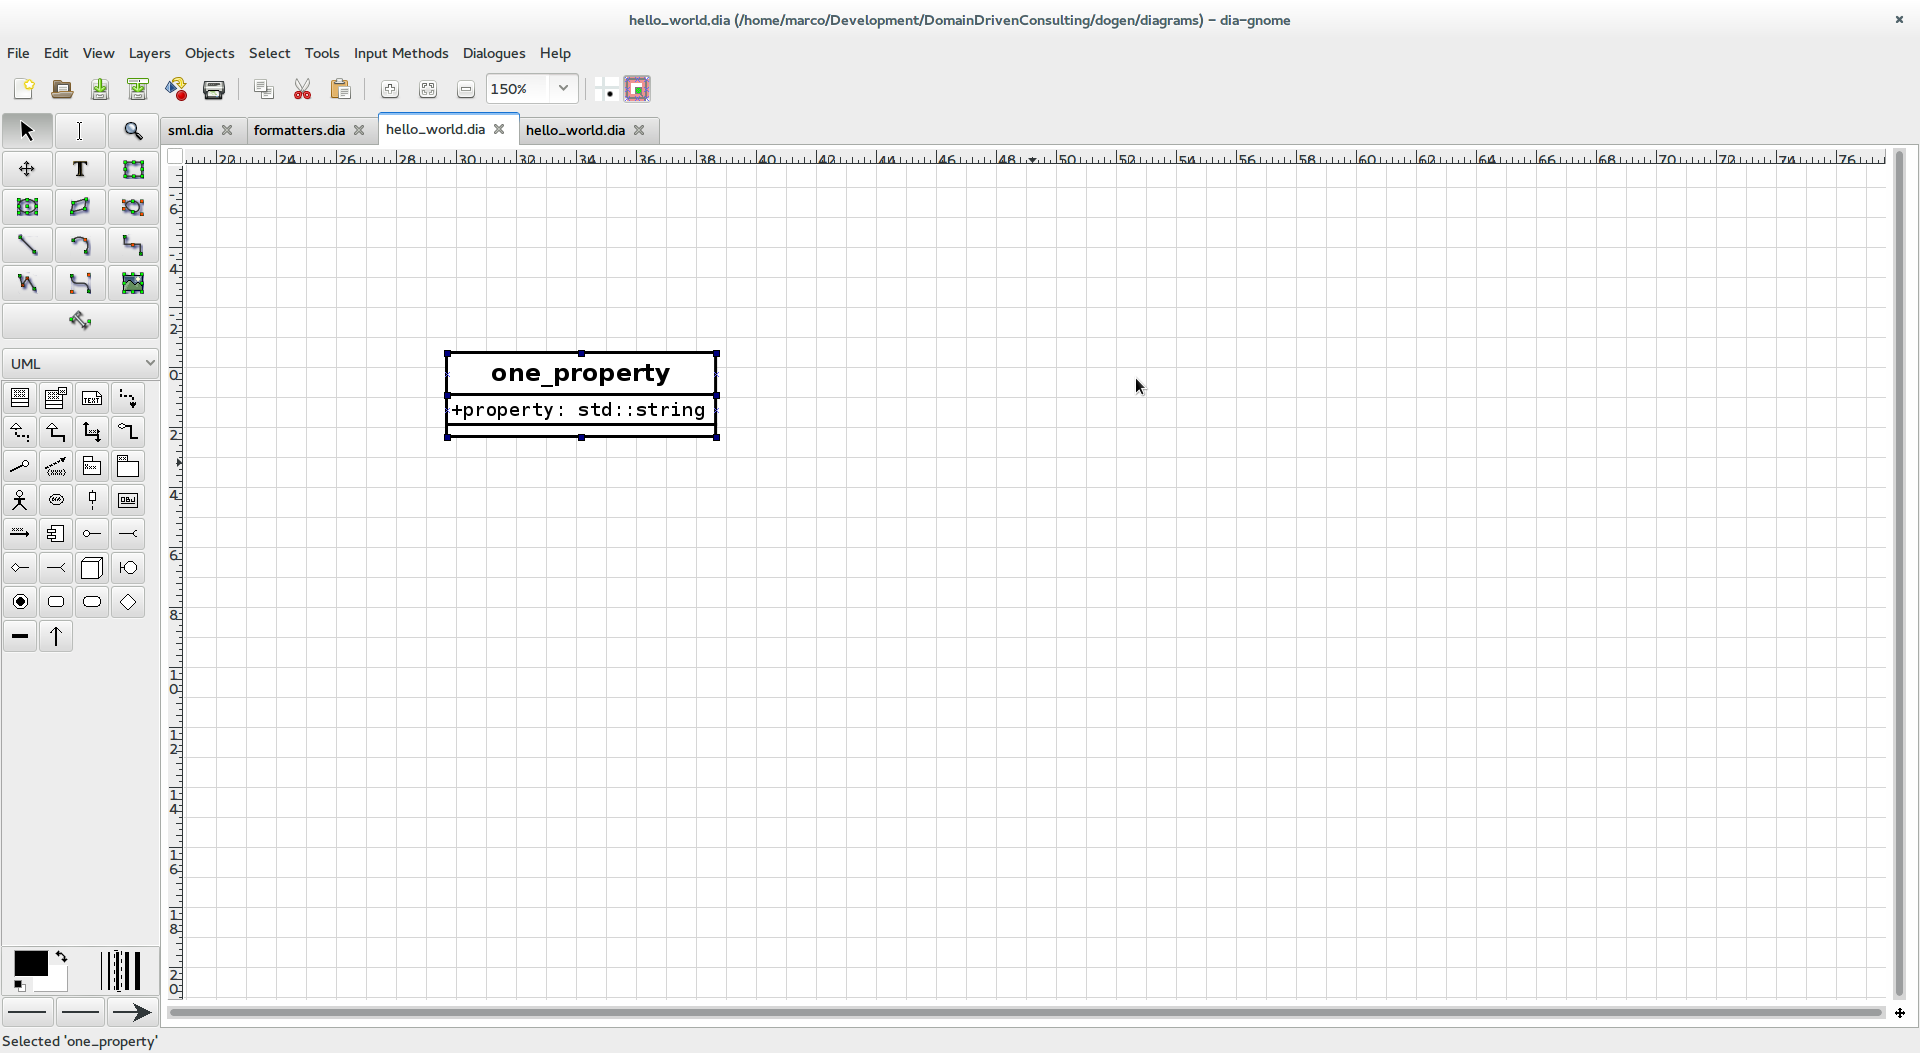
\includegraphics[scale=0.2]{images/dia_hello_world_diagram.png}
    \caption{}
\end{figure}

Feel free to add any comment you'd like to the class; for instance, we
added ``Welcome to Dogen!'', followed by a bit of a blurb about Hello
World.

\begin{figure}[H]
    \centering
    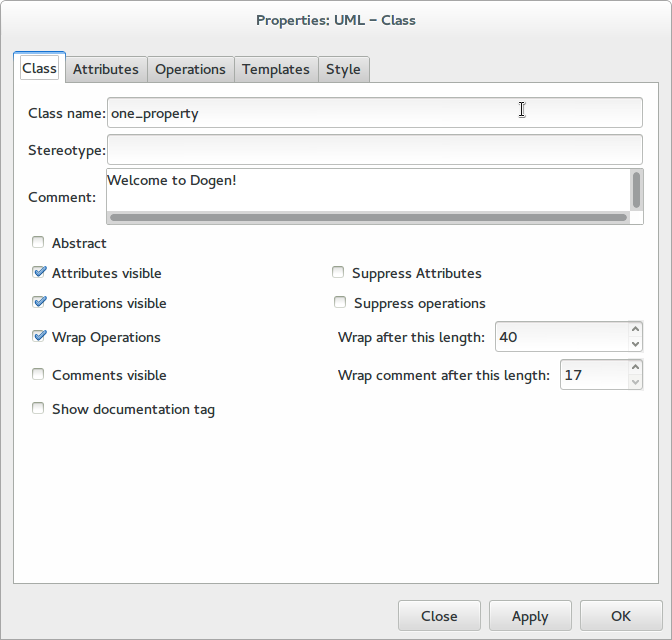
\includegraphics[scale=0.4]{images/dia_hello_world_class.png}
    \caption{}
\end{figure}

Also, make sure you add a property called \texttt{property} to the
class, and give it the type \texttt{std::string}.

\begin{figure}[H]
    \centering
    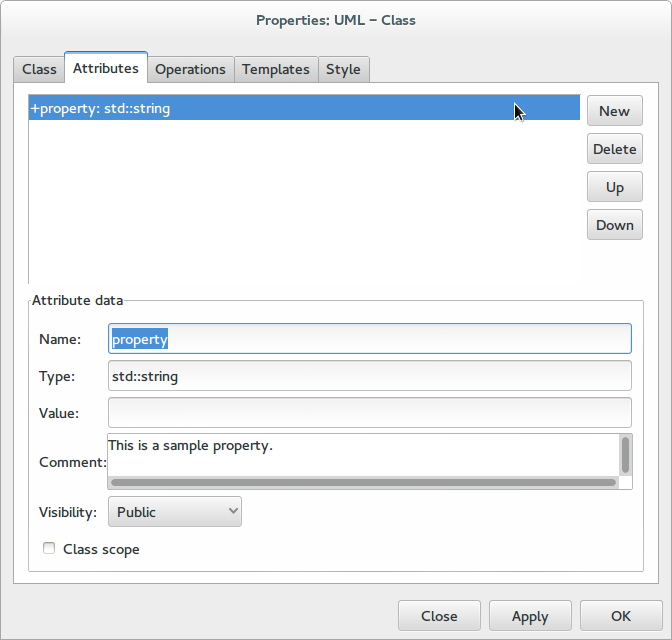
\includegraphics[scale=0.4]{images/dia_hello_world_attributes.png}
    \caption{}
\end{figure}

This diagram is now ready for generation, as described in section
\href{https://github.com/DomainDrivenConsulting/dogen/blob/master/doc/manual/manual.org#generating-hello-world}{Generating
  Hello World}.

\section{UML Types and Their Roles}

Dogen does not support every single UML construct; in fact, it only
supports a surprisingly small subset of the language, but this subset
is rich enough to express all of Dogen's internal complexity. The
supported UML types, according to their Dia names, are described in
the following sections.

\paragraph{UML Class}

The UML Class defines a class, its properties and methods, its
documentation, and all of the associated meta-data that allows Dogen
to treat it specially. For example, depending on the stereotype you
set, a UML Class can be code-generated as a simple value object, an
enumeration or an exception. The following table lists all of the
available stereotypes:

\begin{center}
\begin{tabular}{ll}
Stereotype & Description\\
\hline
service & No code is generated for the class.\\
enumeration & The class is generated as an enumeration.\\
exception & The class is generated as an exception class\\
concept & The class is a ``meta-class''\\
visitable & An associated visitor is created for the class.\\
entity & The class is expected to have an identity.\\
aggregate root & The class is the root of an aggregate.\\
 & \\
\end{tabular}
\end{center}

Some of the above meanings are taken from Domain Driven Design:
service, entity, aggregate root. The remaining ones are convenience
facilities that were added to Dogen. Note that \texttt{visitable} only
makes sense in the presence of inheritance, as explained
\href{https://github.com/DomainDrivenConsulting/dogen/blob/master/doc/manual/manual.org#uml-generalization}{below},
and must be applied to the base class of an inheritance tree.

\paragraph{UML Large Package}

A large package is a container of packages and classes. Dogen uses the
package to define the appropriate scoping in the backend
languages. For example, in C++ it results in placing the contained
types in namespaces.

Note that in Dia it is not possible to add documentation to a
package. This is solved by extending the UML Note, as explained
\href{https://github.com/DomainDrivenConsulting/dogen/blob/master/doc/manual/manual.org#uml-note}{below}.

\begin{figure}[H]
    \centering
    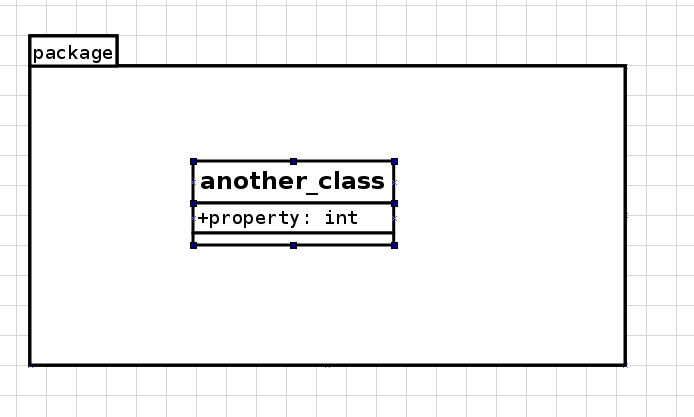
\includegraphics[scale=0.4]{images/class_in_package.png}
    \caption{}
\end{figure}

\paragraph{UML Generalization}

The UML Generalization is used to define inheritance relationships. A
class can have many descendents; however, we do not support multiple
inheritance at present.

\begin{figure}[H]
    \centering
    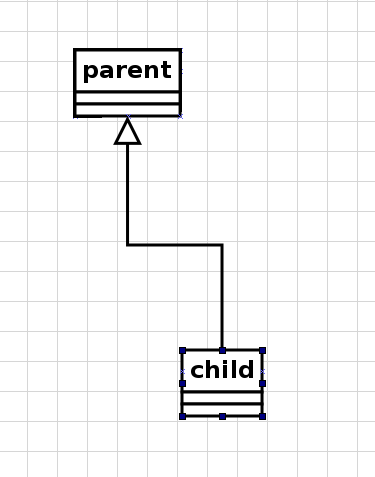
\includegraphics[scale=0.4]{images/generalization.png}
    \caption{}
\end{figure}

\paragraph{UML Association}

The UML Association is used for informational purposes only; Dogen
ignores all UML Associations (either aggregation or composition)
because it does not have enough information to model them. Instead, it
relies on the properties defined in the class to determine
relationships between classes. However, we still find it very useful
to convey graphical meaning to other users of the diagram.

\begin{figure}[H]
    \centering
    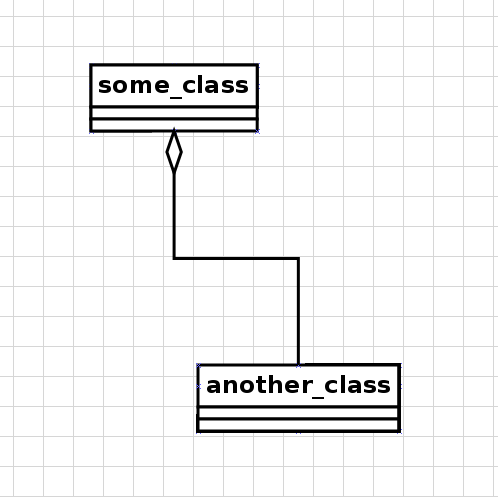
\includegraphics[scale=0.4]{images/association_aggregation.png}
    \caption{}
\end{figure}

\begin{figure}[H]
    \centering
    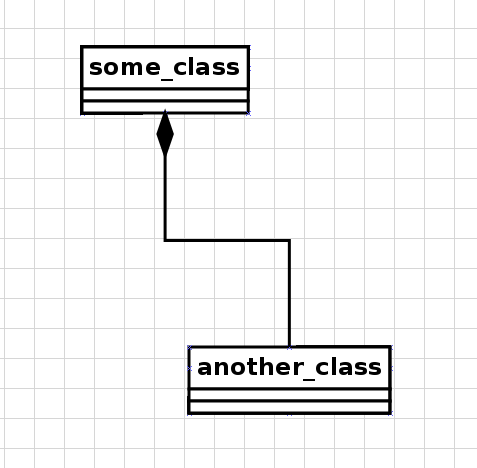
\includegraphics[scale=0.4]{images/association_composition.png}
    \caption{}
\end{figure}

\paragraph{UML Note}

As with standard UML diagrams, the UML Note is used to provide user
comments that clarify intent, add deeper explanations to design
choices and so on. In Dogen, we have overloaded it to supplement
Dia. The main use case is a lack of comments at the model and package
level, which means one could not produce documentation for these
types. We make use of the UML Note to provide this information, by
marking it with meta-data.

\begin{figure}[H]
    \centering
    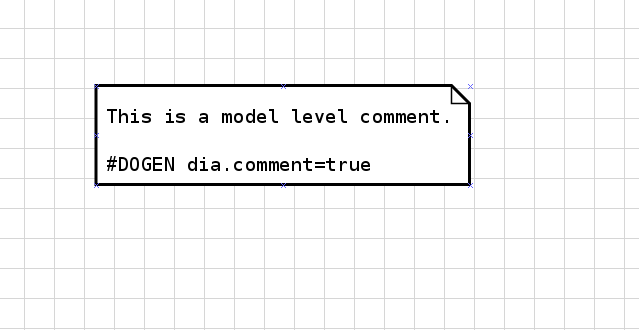
\includegraphics[scale=0.4]{images/model_level_comment.png}
    \caption{}
\end{figure}

\begin{figure}[H]
    \centering
    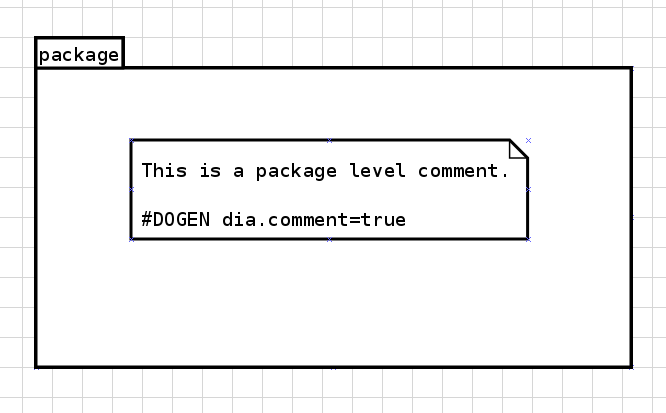
\includegraphics[scale=0.4]{images/package_level_comment.png}
    \caption{}
\end{figure}

\paragraph{UML Message}

The UML Message has, somewhat incorrectly, been overloaded by Dogen as
a way to link comments with classes and other UML types. For instance,
it is useful when you have many classes but you need to provide a UML
Note specific to a class; in that case you can define a UML Message
between the UML Note and the UML Class.

\paragraph{UML realization}

The UML realization is ignored by Dogen. It is useful when you want to
implement interfaces but you do not want Dogen to generate the usual
inheritance infrastructure~--- as it would do if you use a UML
Generalization.

\paragraph{Other Dia object types}

Note that if you attempt to use any other Dia type~--- UML or
otherwise~--- Dogen will fail to process the document and throw an
error. For example, if you try to use the Standard Line you will see
the following in the log file:

\begin{pseudocode}[backgroundcolor=\color{lightgray}]
2014-09-10 08:09:43.480906 [ERROR] [dia_to_sml.processor] Invalid value for object type: Standard - Line
\end{pseudocode}

This strict behaviour was done to avoid subtle bugs. It may be relaxed
in the future as use cases demand it.

\section{Supported Types}

You couldn't fail to notice that we made use of the type
\texttt{std::string}, provided by the C++ Standard Library. This is a
type that is not

\section{Todo}

FIXME: we need to add a section on the supported object types and the
handling of unsupported object types.

\begin{itemize}
\item Properties
\item Comments
\item Packages
\item Association
\item Inheritance: same model, across models.
\item Enumerations
\item System Models: JSON format, Standard C++ System Model, Boost System Model
\end{itemize}

\chapter{Frequently Asked Questions}

\textbf{Q}: When I tried running Dogen I get the following error
message:

\begin{pseudocode}[backgroundcolor=\color{lightgray}]
Error: File not found: Could not find data directory.
Base directory: /A/FULL/PATH. Locations searched: ./data ../data ../share/data
See the log file for details: 'log/dogen_knitter_MODEL_NAME.log'
Failed to generate model: 'MODEL_NAME'.
\end{pseudocode}

\textbf{A}: Your installation of Dogen is faulty. This could happen
for example if you copy the Dogen binary from a build directory into
another location without copying all the associated
infrastructure. The correct way is to run the binary using a relative
path to the build directory: \texttt{../../dogen\_knitter}.

This error should not occur if you are using a binary package as the
binary should be in the system path.

\textbf{Q}: I get the error ``Invalid value for object type'' when
generating; what does that mean?

You have tried to use a Dia object type that is not supported by
Dogen. Locate the object type and remove it from your diagram. For a
list of supported object types see FIXME.

\appendix

\chapter{Related Work}

This section is a bit of a general research bucket. It contains a set
of links to the C++ code generators we have found on our wanderings on
the internet, as well as other interesting projects in this space~---
including those in other programming languages. It also contains books
and papers on the subject we have read, or intend to read.

\begin{itemize}
\item
  \href{http://www.amazon.co.uk/Domain-Driven-Design-Tackling-Complexity-ebook/dp/B00794TAUG/ref\%3Dsr_1_2?ie\%3DUTF8&qid\%3D1368380797&sr\%3D8-2&keywords\%3Dmodel\%2Bdriven\%2Bdesign}{Domain-Driven
    Design: Tackling Complexity in the Heart of Software}: The Eric
  Evans book from which we tried to steal most concepts in Dogen. A
  must read for any developer.
\item
  \href{http://www.amazon.co.uk/EMF-Eclipse-Modeling-Framework-ebook/dp/B0013TPYVW/ref\%3Dsr_1_2?s\%3Dbooks&ie\%3DUTF8&qid\%3D1368380262&sr\%3D1-2&keywords\%3DEclipse\%2BModeling\%2BFramework\%2B\%255BPaperback\%255D}{EMF:
    Eclipse Modeling Framework}: The original EMF book. Useful read
  for anyone interested in code generation.
\item
  \href{http://www.scribd.com/doc/78264699/Model-Driven-Architecture-for-Reverse-Engineering-Technologies-Strategic-Directions-and-System-Evolution-Premier-Reference-Source}{Model
    Driven Architecture for Reverse Engineering Technologies}: Preview
  of a potentially interesting MDA book.
\item
  \href{http://www2.informatik.hu-berlin.de/~piefel/Documents/06CITSA-CMMCG.pdf}{A
    Common Metamodel for Code Generation}: This paper will be of
  interest if we decide to support multiple languages.
\item
  \href{http://www.vollmann.com/pubs/meta/meta/meta.html}{Metaclasses
    and Reflection in C++}: Some (early) ideas on implementing a MOP
  (Meta Object Protocol) in C++.
\item
  \href{https://code.google.com/a/eclipselabs.org/p/cppgenmodel/}{cppgenmodel
    - A model driven C++ code generator}: This seems more like a run
  time / reflection based generator.
\item \href{https://code.google.com/p/emf4cpp/}{EMF4CPP - Eclipse
  Modeling Framework}: C++ port of the EMF/eCore eclipse framework. As
  with Java it includes run time support. There is also
  \href{http://apps.nabbel.es/dsdm2010/download_files/dsdm2010_senac.pdf}{a
    paper} on it.
\item
  \href{http://www2.informatik.hu-berlin.de/~piefel/Documents/06CITSA-CMMCG.pdf}{A
    Common Metamodel for Code Generation}: Describes a meta-model
  designed to model Java and C++.
\item
  \href{http://marofra.com/oldhomepage/MetaCPlusPlusDoc/metacplusplus-1.html}{The
    Meta-C++ User Manual}: Another early C++ meta-modeling
  tool. Contains interesting ideas around C++ meta-models.
\item The Columbus C++ Schema: Useful tool for re-engineering large
  C++ code bases. Contains a meta-model for C++. A number of papers
  have been written about it:
\begin{itemize}
\item
  \href{http://www.inf.u-szeged.hu/~beszedes/research/tech27_ferenc_r.pdf}{Columbus
    – Reverse Engineering Tool and Schema for C++}
\item
  \href{http://journal.ub.tu-berlin.de/eceasst/article/download/10/19}{Third
    Workshop on Software Evolution through Transformations}: Embracing
  the Change
\item
  \href{http://www.inf.u-szeged.hu/~ferenc/research/ferencr_schema.ppt.pdf}{Towards
    a Standard Schema for C/C++}
\item
  \href{http://www.inf.u-szeged.hu/~ferenc/research/ferencr_columbus_schema_cpp.pdf}{Data
    Exchange with the Columbus Schema for C++}
\end{itemize}
\item \href{http://www.cpgf.org/}{CPGF}: An open source C++ library
  for reflection, script binding, serialisation and callbacks.
\item \href{http://www.artima.com/articles/dci_vision.html}{DCI}: The
  DCI Architecture: A New Vision of Object-Oriented Programming. Some
  fundamental insights on the nature of OO.
\item \href{http://www.ischo.com/xrtti/index.html}{xrtti}: Extending
  C++ with a richer reflection.
\item
  \href{http://www.open-std.org/jtc1/sc22/wg21/docs/papers/2014/n3883.html}{Code
    checkers and generators}: adding AngularJS-like capabilities to
  C++.
\item
  \href{http://stackoverflow.com/questions/355650/c-html-template-framework-templatizing-library-html-generator-library}{Text
    Template libraries for C++}: T4 like implementations for C++.
\item The XML binding tools:
  \href{http://msdn.microsoft.com/en-us/library/x6c1kb0s(v\%3Dvs.110).aspx}{Xsd
    tool}, \href{http://www.codesynthesis.com/products/xsd/}{xsd for
    c++}, \href{https://jaxb.java.net/2.2.4/docs/xjc.html}{xjc}, etc
  provide ideas on code generation and can be used to generate plain
  domain objects.
\end{itemize}

\chapter{Assorted Text}

The main objective of creating a domain generator is to avoid having
to maintain manually a significant amount of trivial code; this not
only speeds up the development process but it also improves code
quality as programmers do not tend to perform repetitive tasks
terribly well.

We developed our own domain generator because we could not find one
that fitted our requirements~--- open source or otherwise. You can see
the results of our research
\href{https://github.com/kitanda/dogen/blob/master/doc/manual/manual.org#appendix-a---related-work}{in
  the manual's appendix}.

Note that Dogen is specifically tailored for our needs. We are,
however, wiling to accept any patches for functionality not directly
required by us.

\backmatter
\bibliographystyle{plain}
\bibliography{manual}

\end{document}
